%%%%%%%%%%%%%%%%%%%%%%%%%%%%%%%%%%%%%%%%%%%%%%%%%%%%%%%%%%%%%%%%%%%%%%%%%%%%
%% CR-SHE v5: Elsevier CAS single-column template (cas-sc).
%% v5 merges an externally edited v5 and a reviewed v4 (ChatGPT/Gemini) with v4;
%% see docs/DRAFT_AUDIT_v5.md for every change accepted, corrected or rejected.
%%
%% REVISION MARKERS. \authorcheck{...} prints a red note for the authors: an
%% experiment or full-text check still to be done. Every marker must be resolved
%% before submission. Set \authorcheckstrue to see them.
%% Guide for authors checked October 2026: abstract <= 250 words, 1-7 keywords,
%% 3-5 highlights of <= 85 characters (also supplied as a separate file),
%% single-anonymized review, CRediT, research-data Option C, AI declaration
%% placed before the references.
%%
%% Build:  pdflatex -> bibtex -> pdflatex -> pdflatex
%%
%% House-style notes for this file
%%   * No em dashes anywhere in the text. Parenthetical asides use
%%     commas, colons, semicolons or parentheses instead. The double hyphen
%%     (--) appears only as an en dash inside numeric ranges, which is the
%%     Elsevier convention for ranges.
%%   * Fig. 1 (the architecture) is a full-text-width figure* float; it is
%%     regenerated by figures_src/fig_architecture.py.
%%%%%%%%%%%%%%%%%%%%%%%%%%%%%%%%%%%%%%%%%%%%%%%%%%%%%%%%%%%%%%%%%%%%%%%%%%%%

% Single column: the journal's default layout and easier for reviewers.
\documentclass[a4paper,fleqn]{cas-sc}

\usepackage[numbers,sort&compress]{natbib}
\usepackage{algorithm}
\usepackage{algpseudocode}
\usepackage{placeins}   % keep floats out of the back matter

% Let a tight line stretch rather than spill into the neighbouring column.
\setlength{\emergencystretch}{3em}

% amssymb (loaded by cas-dc) supplies \checkmark; this is a harmless guard in
% case a future font package withdraws it.
\providecommand{\checkmark}{\ensuremath{\surd}}


% ANONYMIZED BUILD. The submission system asks for a manuscript without
% author details plus a separate title page.
%   \anonymoustrue   -> manuscript without author details (upload this)
%   \anonymousfalse  -> full version with authors, CRediT and highlights page
% \input is not expandable, so it cannot open a tabular row that starts with
% \multicolumn or a rule; the TeX primitive can.
\makeatletter\let\inputtbl\@@input\makeatother

\newif\ifanonymous
\anonymoustrue
% the class prints an "ORCID(s):" footnote even when no author is given
\ifanonymous\RenewDocumentCommand\printorcid{}{}\fi

% Open items for the authors (hidden in the submission build).
\newif\ifauthorchecks
\authorchecksfalse   % submission build; set \authorcheckstrue to see open items
\newcommand{\authorcheck}[1]{\ifauthorchecks{\color{red}\textsf{[Authors: #1]}}\fi}


% Theorem-like environments, using the constructs cas-dc provides.
\newtheorem{theorem}{Theorem}
\newtheorem{lemma}{Lemma}
\newtheorem{proposition}{Proposition}
\newdefinition{definition}{Definition}
\newdefinition{remark}{Remark}
\newproof{pf}{Proof}

\newcommand{\negl}{\mathsf{negl}}
\newcommand{\PPT}{\mathrm{PPT}}
\newcommand{\Real}{\mathbf{Real}}
\newcommand{\Ideal}{\mathbf{Ideal}}
\newcommand{\Leak}{\mathcal{L}}
\newcommand{\Sim}{\mathcal{S}}
\newcommand{\Adv}{\mathcal{A}}
\newcommand{\cind}{\approx_c}
\newcommand{\Gen}{\mathsf{Gen}}
\newcommand{\Eval}{\mathsf{Eval}}
\newcommand{\Setupp}{\mathsf{Setup}}
\newcommand{\BuildIndex}{\mathsf{BuildIndex}}
\newcommand{\EncData}{\mathsf{EncData}}
\newcommand{\Token}{\mathsf{Token}}
\newcommand{\Search}{\mathsf{Search}}
\newcommand{\Compute}{\mathsf{Compute}}
\newcommand{\Dec}{\mathsf{Dec}}
\newcommand{\Enc}{\mathsf{Enc}}
\newcommand{\advPRF}{\mathbf{Adv}^{\mathrm{prf}}}
\newcommand{\advDPF}{\mathbf{Adv}^{\mathrm{dpf}}}
\newcommand{\advCPA}{\mathbf{Adv}^{\mathrm{cpa}}}
\newcommand{\bplus}{\boxplus}
\newcommand{\bminus}{\boxminus}
\newcommand{\bdot}{\boxdot}

\begin{document}
\let\WriteBookmarks\relax
\def\floatpagepagefraction{1}
\def\textpagefraction{.001}

\shorttitle{Tamper-evident oblivious range analytics over encrypted IoT data}
\ifanonymous\shortauthors{Anonymous authors}\else\shortauthors{M. M. Islam et~al.}\fi

\title[mode=title]{CR-SHE: One-round, tamper-evident range analytics over
encrypted, replicated IoT data under $(n{-}1)$-collusion}

\ifanonymous\else
%% ===========================================================================
%% Authors
%% ===========================================================================
\author[1]{Md Mazharul Islam}[orcid=0000-0001-6225-1487]
\cormark[1]
\ead{mazharul.islam1@northsouth.edu}
\credit{Conceptualization, Methodology, Software, Formal analysis,
Investigation, Validation, Writing -- original draft,
Writing -- review and editing}

\author[1]{Mubasshir Ahmed}[orcid=0000-0002-7502-3835]
\ead{mubasshir.ahmed@northsouth.edu}
\credit{Software, Data curation, Investigation,
Writing -- review and editing}

\author[1]{Md Redowan Zaman Anik}
\ead{redowan.anik@northsouth.edu}
\credit{Software, Data curation, Visualization, Validation,
Writing -- review and editing}

\affiliation[1]{organization={Department of Electrical and Computer
    Engineering, North South University},
    city={Dhaka},
    country={Bangladesh}}

\cortext[cor1]{Corresponding author.}
\fi

%% ===========================================================================
%% Abstract
%% ===========================================================================
\begin{abstract}
Hiding which records an encrypted IoT query touches is worthless if
aggregating over them hands the matched set back to the servers.
We present CR-SHE, which answers multi-dimensional range aggregates over data
encrypted under one owner's key and replicated to $n$ providers, in one round
without communication between providers, hiding the range, the matched
records, their number and the result from any coalition of up to $n-1$
semi-honest providers. The owner stores encrypted summed-area tables of
registered data cubes; a query is $2^d$ distributed-point-function keys with
signed outputs at the box's corners, padded with dummy keys, and each provider
returns one ciphertext. A second key set carries a secret scalar chosen afresh
for every query, so an honest client accepts a wrong answer with probability
about $2^{-36}$ whatever deviating providers compute, with no stored MAC key and no
extra homomorphic work. Role-scoped columns and mask keys confine each user to
its own role's records. On two real IoT corpora totalling $825{,}554$ records
a C++ prototype answers single-keyword aggregates in $39$\,ms per provider. In
a reference implementation on a synthetic cube of $345{,}690$ cells with the
real corpus's dimensions, range cost and the $132$\,kB response stay flat from
a one-minute window to the whole timeline, and no wrong answer was accepted in
$4{,}000$ tampered trials. A verified query uploads $5{,}520$ bytes per
provider, against a computed $44$\,MB for a plain single-server baseline.
\end{abstract}

%% ===========================================================================
%% Highlights (each line is kept under 85 characters, as Elsevier requires)
%% ===========================================================================
% Highlights are uploaded as a separate file; the class prints the author list
% on the highlights page, so it is omitted from the anonymized build.
\ifanonymous\else
\begin{highlights}
\item One-round range aggregates over encrypted IoT data, hidden from n-1 clouds.
\item Encrypted summed-area tables turn any d-dimensional box into 2^d DPF keys.
\item A fresh secret scalar in each query makes provider tampering evident.
\item Role-scoped columns and mask keys confine each user to its own records.
\item Cost and the 132 kB response are flat from one minute to the whole timeline.
\end{highlights}
\fi

\begin{keywords}
Range aggregation \sep
Distributed point function \sep
Homomorphic encryption \sep
Internet of Things \sep
Multi-cloud \sep
Summed-area table \sep
Verifiable computation
\end{keywords}

\maketitle

% ===========================================================================
\section{Introduction}
\label{sec:intro}

The proliferation of connected sensors, wearables and cyber-physical systems
has made the Internet of Things (IoT) one of the largest and fastest-growing
sources of continuously generated data \citep{atzori2010internet}. Bedside
monitors, smart meters, traffic and environmental sensors and industrial
controllers emit measurements continuously, and the people who need to query
them, among them clinicians, grid operators, city agencies and maintenance
contractors, are rarely the ones who own the devices. The natural response is
to serve this data from the cloud, and modern deployments increasingly
replicate it across several providers. Multi-cloud operation supplies elastic
query capacity, improves availability through redundancy across independent
infrastructures, and frees data owners from single-vendor lock-in
\citep{petcu2013multicloud,grozev2014intercloud}. Yet much of this data is
acutely sensitive, including physiological telemetry in connected healthcare,
mobility traces in smart cities and diagnostic streams from connected
vehicles, so it must be encrypted before leaving the IoT trust domain and stay
encrypted in the cloud, even as multiple stakeholders need to query and
analyse it.

Encrypting outsourced data with conventional schemes neutralises the reason it
was sent to the cloud. A provider holding only ciphertexts can neither locate
the records a query needs nor compute over them, forcing either decryption in
the cloud, which reintroduces exposure, or a wholesale download to the client,
which defeats the purpose of outsourcing. Searchable encryption lets a
provider identify records matching an encrypted keyword
\citep{song2000practical,curtmola2006searchable,islam2023keyword}, and leveled
homomorphic encryption lets it evaluate bounded-depth arithmetic directly on
ciphertexts \citep{fan2012somewhat,cryptoeprint:2016/421}. Both, in their
single-server form, leak the access pattern, and a substantial body of
leakage-abuse work converts that leakage into plaintext recovery
\citep{islam2012access,cash2015leakage,grubbs2017leakage}.

Replicating data across independent providers offers an escape that
single-server cryptography cannot. If the client splits its query so that no
provider sees it, the access pattern stays hidden as long as one provider
abstains from collusion. Splinter \citep{splinter} established this model with
function secret sharing, DORY \citep{dory} brought it to encrypted documents,
and Waldo \citep{waldo} extended it to rich predicates over time series. The
model is therefore not new. What remains open is narrower: moving from private
selection to encrypted, multi-dimensional range analytics without handing the
selection back to the servers.

\emph{Selection and computation are not the same problem, and hiding the first
is worthless if the second gives it back.} A scheme can privately determine
which records match a keyword and then, in order to aggregate over them, hand
the matched index set to the providers, at which point the coalition learns
the access pattern exactly, and across repeated queries the search pattern. We
call this the \emph{selection-to-computation composition leak}. Existing
distributed-trust systems avoid it by not computing at all (DORY), by
computing over data the servers can already read (Splinter, whose databases
are public), by moving to a three-party honest-majority setting with
secret-shared data and server-to-server interaction (Waldo), or by
evaluating predicates over Shamir shares of unary-encoded values without server
interaction (Obscure \citep{gupta2019obscure,gupta2020obscure}), where
multiplying shares raises the polynomial degree and with it the number of
servers needed for a given collusion bound.\authorcheck{Confirm against the
Obscure full text the exact relation between servers, predicate length and
collusion threshold, and state it here.} Multi-cloud IoT deployments add three
constraints that together define our setting: (i) privacy must hold while any
one provider is honest, $t=n-1$; (ii) providers never talk to one another, so
there are no cross-cloud channels, synchronisation or egress charges; and
(iii) the data are encrypted once under the owner's key, so a replica can be
added, lost or revoked by copying ciphertexts, without re-dealing shares.
These constraints rule out the obvious alternative of secret-sharing the data
at $t=n-1$, because a shared store cannot answer a hidden query without either
server interaction or a single-server private-retrieval primitive
(Section~\ref{sec:whyrep}).

\emph{IoT analytics are range queries.} A clinician asks for one patient's
mean heart rate across a night, a city agency for the number of hours carbon
monoxide sat in its top three bands at one site, a maintenance contractor for a
machine's vibration total over a shift. Each is an aggregate over a box in a
small number of ordered dimensions: device, time window, value band. Answering
such a box with single-keyword aggregates costs one query per tag in the box
and reveals its length; retrieving the records first costs a retrieval per tag
and hands the client data it did not ask for. Prior distributed-trust systems
that support ranges compute over plaintext or need an honest majority with
interaction (Section~\ref{sec:related}), and single-server encrypted range
aggregation leaks access patterns or evaluates homomorphic comparisons.

We propose CR-SHE (Collusion-Resilient Searchable Homomorphic Encryption). The
data owner replicates a one-time-pad-masked pseudonymous index and a
homomorphically encrypted record column to $n$ providers. A registered
single-keyword query sends one distributed point function (DPF) key per
provider, and a registered $d$-dimensional range sends $2^d$. Rather than
returning the selection vector so the client can name the matched records, each
provider contracts its \emph{own share} of that vector against owner-encrypted
columns and returns a single ciphertext; the client adds the $n$ ciphertexts
and decrypts once. The matched set is never assembled at any provider, its cardinality
never leaves the client, and per-query downlink for an aggregate is one
ciphertext rather than linear in the record count. The contributions are as
follows.

\begin{itemize}
\item \textbf{One-round oblivious range aggregation} (Section~\ref{sec:range}).
The owner registers data cubes over ordered tag families and stores encrypted
summed-area tables. A $d$-dimensional box query is $2^d$ DPF keys with signed
outputs at its corners, padded with zero-output dummy keys so that ranges
touching the cube's edge are indistinguishable, and each provider returns one
ciphertext. Provider work and the response are independent of the range and of
the record count; cost is linear in the cube's size.

\item \textbf{Tamper evidence from a per-query secret}
(Section~\ref{sec:verify}, Theorem~\ref{thm:tamper}). Each column's second slot
row holds a copy of its first, and the client sends a second key set whose
outputs carry a fresh secret scalar $\delta_s$. Whatever a coalition of
providers computes, the client accepts a changed answer with probability at
most $1/(p-1)$ plus the DPF advantage, on every path: single keyword, range and
the flexible path. No MAC key is stored, the homomorphic work is unchanged, and
the deviations that per-row and per-cell keys miss, those aimed at the queried
point, are caught. A one-time MAC key chosen by the client already appears in
two-server decision-tree evaluation \citep{li2026silent}, delivered under
homomorphic secret sharing; what is specific here is carrying it inside the DPF
outputs, at no public-key or homomorphic cost, and an argument that covers
coalitions of up to $n-1$ providers.

\item \textbf{Role-scoped access without interaction} (Section~\ref{sec:auth}).
A user of one role holds only that role's mask key, so retrieval reveals
membership bits of its own records and leaves the rest one-time-padded; its
aggregate columns, cube tables and record column are built from its records
only, so no vector it sends reaches another role's data. Providers apply a
role-to-column policy and nothing else. This turns the authorisation gap of our
earlier design into a stated mechanism, at a storage cost per role.

\item \textbf{The composition leak, and the cost of avoiding a homomorphic
layer at $t=n-1$.} Proposition~\ref{prop:nolocal} shows that local answers over
$(n,n)$ additive shares miss cross terms, and that a non-interactive repair with
data-independent queries, correct on every share tuple, yields single-server
private information retrieval, hence oblivious transfer. This is not a lower
bound for every secret-sharing design: threshold sharing at a lower collusion
bound, preprocessing or interaction escape it, and the homomorphic layer is our
design choice at $t=n-1$.

\item \textbf{The single-keyword fast path, packing and a flexible path.}
Registered single-keyword templates cost a symmetric full-domain pass plus
$O(N/\ell)$ packed ciphertext operations, independent of the record count, with
several templates in the two slot rows of one ciphertext; a two-round flexible
path serves conjunctions and ad-hoc weights; the masked membership index is
one-time-padded and packed $32$ bits per word, an engineering step that cuts it
$32$-fold. The algebraic compatibility condition (Lemma~\ref{lem:compat}) under
which DPF shares and the homomorphic plaintext ring compose is made explicit.

\item \textbf{Evaluation and its scope.} A C++ prototype measured the
single-keyword path, a single-host multi-provider deployment, six baselines and
a leakage-abuse attack on two real IoT corpora totalling $825{,}554$ records
and $46{,}742$ tags. A reference implementation measures range aggregation on a
synthetic cube with the primary corpus's dimensions, all three verification
modes against five injected deviations ($4{,}000$ session-check trials), the
role-scoped extraction attack and the packed index
(Section~\ref{sec:resultsdisc}). Range aggregation on the real corpora, a
native port and a cross-region deployment remain to be measured.
\end{itemize}

The remainder of this paper is organised as follows.
Section~\ref{sec:related} reviews related work. Section~\ref{sec:prelim} fixes
notation and primitives. Section~\ref{sec:system} presents the system and
threat model. Section~\ref{sec:construction} details
the construction, Section~\ref{sec:security} the security analysis, and
Section~\ref{sec:complexity} the asymptotic costs. Section~\ref{sec:impl}
describes the implementation, Section~\ref{sec:resultsdisc} reports and
discusses results, and Section~\ref{sec:conclusion} concludes.

% ===========================================================================
\section{Related work}
\label{sec:related}

\subsection{Distributed-trust query systems}
Splinter \citep{splinter} established the model of splitting a query into
function-secret-sharing shares evaluated against replicas, hidden as long as
one provider abstains, with \textsc{sum}, \textsc{count}, \textsc{max} and
\textsc{topk} over \emph{public} cleartext databases. Its conditions are
equalities, intervals, and an AND of equalities with at most one interval
\citep[Fig.~4]{splinter}, so it answers one-dimensional range aggregates over
public data; its providers are honest-but-curious, and it does not protect
against incorrect results \citep[\S2.3]{splinter}. DORY \citep{dory} moves to
encrypted documents: $\ell$ replicas ($\ell=2$ in its implementation) hold a
Bloom-filter index whose bits are one-time-padded with a PRF of a per-folder
key and the document version \citep[\S4.1]{dory}; it hides search access
patterns, including the number of results, from an attacker that maliciously
controls $\ell-1$ of the $\ell$ trust domains, and proves security with abort
using aggregate MACs \citep[\S3.4, \S4.3]{dory}. It stops at retrieval. Waldo \citep{waldo} supports multi-predicate filtering over
time series with malicious security, in a three-party honest-majority setting
with secret-shared data and server-to-server interaction, that is, a
collusion bound of $t=1$. CR-SHE trades Waldo's predicate expressiveness and
full malicious security for $t=n-1$, no inter-provider communication and
owner-keyed encryption at rest. Obscure \citep{gupta2019obscure,gupta2020obscure}
is the closest system we found: aggregation queries with conjunctive or
disjunctive predicates over Shamir secret-shared, unary-encoded data, hiding
access and query patterns, without communication between servers and with
optional result verification. Because evaluating a predicate multiplies shares,
the polynomial degree grows with the predicate, and one-round evaluation needs
correspondingly more servers per tolerated colluder. Against it CR-SHE offers
$t=n-1$ for any $n\ge2$, owner-encrypted replicas that need no re-dealing, and
range aggregation with a fixed $2^d$ keys per box. We have read Obscure's
abstracts and search summaries of its full version, not the full text, so we
do not state its exact thresholds or its range mechanism.\authorcheck{Read the
Obscure full version (arXiv 2004.13115) and replace this paragraph with its
exact server and threshold requirements, range support and verification.} The primitives are due to Gilboa and Ishai
\citep{gilboa2014distributed} and Boyle, Gilboa and Ishai
\citep{boyle2015function,boyle2016function}; FSS also serves metadata-hiding
messaging \citep{express}, robust private statistics
\citep{corrigan2017prio,boneh2021lightweight}, access control for dealers
\citep{pacl} and verifiable keys \citep{decastro2022lightweight}; fast
FSS-based secure computation \citep{storrier2023grotto} and DPF-based ORAM for
secure computation \citep{doerner2017scaling} are complementary to the
ciphertext-side contraction below. At bottom, DPF-based selection is
multi-server PIR \citep{chor1998private}, and its linear server work is the
price of PIR without preprocessing \citep{beimel2000reducing}; what CR-SHE adds
is the ciphertext-side contraction with key-carried session verification, the
packed masked index, and one-round prefix-sum range cubes.

\subsection{Private range aggregation}
Prefix sums answer a range sum from a constant number of lookups, a structure
known from data cubes \citep{ho1997range} and summed-area tables
\citep{crow1984summed}. Boyle, Gilboa and Ishai obtain function secret sharing
for $d$-dimensional intervals with key size $O(\lambda n^d)$ for $n$-bit
coordinates by reducing a box, through inclusion--exclusion, to $2^d$
intervals anchored at zero \citep[Cor.~3.4]{boyle2016function}; the
decomposition our range path uses is therefore theirs, applied on the data side
rather than the function side (Section~\ref{sec:range}). Over encrypted data
held by one server, ARQ \citep{espiritu2022arq} builds range sums, minima,
modes and medians from structured encryption, primarily for one-dimensional
queries; its strongest notion, data obliviousness, still lets the query leakage
depend on the query itself \citep[Def.~3.3]{espiritu2022arq}, and its range-sum
scheme follows Demertzis et al.'s prefix sums \citep{demertzis2018practical}.
HADES \citep{liu2025hades} evaluates point and range predicates under fully
homomorphic encryption in one round at a single server holding public data.
With non-colluding servers, Hayata et al.\ \citep{hayata2020private} give
FSS-based PIR for range \emph{retrieval}; in Hafiz et
al.\ \citep{hafiz2024private} the servers host the database and multiply the
client's Shamir-shared query vector by precomputed aggregate-query indexes,
with a Byzantine-robust variant; and Waldo \citep{waldo} supports range
predicates over secret-shared time series with an honest majority and server
interaction. CR-SHE's range path instead
composes prefix-sum data cubes with oblivious homomorphic contraction, so that
the data remain encrypted at rest under the owner's key, the coalition bound is
$t=n-1$ for any $n\ge 2$, and providers answer $d$-dimensional box queries in
one round without interacting. Neither private aggregation nor prefix-sum range
queries is new in isolation, and function secret sharing for multi-dimensional
intervals exists \citep{boyle2016function}; the contribution is the
combination. We have read Splinter, DORY, ARQ, PVODTE and the FSS
constructions of Boyle et al.\ in full; our characterisation of Obscure, Hafiz
et al., HADES and Hayata et al.\ rests on their abstracts and on search
summaries, so we make no claim of priority; the search log ships with our
artefact.\authorcheck{Update after reading Obscure, Hafiz et al.\ and HADES in
full.}

\subsection{Verification and access control for hidden queries}
Verifiable DPFs \citep{decastro2022lightweight} and access control for FSS
\citep{pacl,ji2023finegrained} let servers check that a client's \emph{keys}
are well formed or authorised; they guard against a malicious client. Against
malicious servers, DORY keeps per-bit MAC tags condensed into aggregate MACs
\citep[\S4.3]{dory}, verifiable homomorphic secret sharing
\citep{choudhuri2024vehss} checks evaluation, and PVODTE \citep{li2026silent}
has the client generate a one-time MAC key, encrypt it under homomorphic secret
sharing and send it to two servers, which return the result alongside its
product with the key \citep[\S VII-B]{li2026silent}; PVODTE is secure against
one malicious server and leaves verifiability against colluding servers to
future work \citep[\S IV-D]{li2026silent}. Our tamper evidence is the same kind
of information-theoretic MAC, value $y$ alongside $\delta_s y$ as in SPDZ
\citep{damgard2012spdz}, with $\delta_s$ drawn afresh per query; it differs in
carrying $\delta_s$ inside the DPF outputs, so the providers' stored state holds
no key and no public-key operation or extra homomorphic product is needed, and
in an argument (Theorem~\ref{thm:tamper}) that covers coalitions of up to
$n-1$ providers. Our role-scoped access restricts which \emph{data} a
query can reach rather than which keys are accepted, and needs no proof or
server-to-server message; it pays in storage per role.

\subsection{Private information retrieval}
PIR with preprocessing breaks the linear lower bound: offline hints let the
online phase run in sublinear time, with two servers
\citep{corrigan2020private} or one \citep{corrigan2022single,zhou2024piano}.
Those hints are client state computed over the whole database and invalidated
by updates, which suits a stable table read by one client better than a stream
ingested continuously and queried by many stateless data users; we keep the
linear pass and list preprocessing as future work. Single-server PIR from
lattice-based encryption
\citep{angel2018pir,mughees2021onionpir,menon2022spiral,davidson2023frodopir}
removes the non-collusion assumption altogether
\citep{kushilevitz1997replication}. For the fast path in isolation it is a
genuine alternative, being a PIR query into a table of owner-encrypted
aggregates, and we measure it directly as baseline~(vi)
(Section~\ref{sec:packing}): on that path one CR-SHE provider does less work
than the single server but two providers together do not, and the trust split
saves three to four orders of magnitude in uplink and $27$--$109$ times in
client computation, not asymptotic work. On retrieval and the flexible path a single server must
multiply an encrypted selection vector by the whole $N\times N_d$ index, at
least $N\lceil N_d/32\rceil/\ell$ homomorphic products with the same bit
packing, which we bound at $1.5$--$3.1$ times CR-SHE's retrieval in the same
implementation; again a constant factor, with the uplink gap on top.

\subsection{Encrypted search, encrypted analytics and multi-cloud storage}
Searchable encryption leaks search and access patterns, which leakage-abuse
attacks turn into plaintext recovery
\citep{islam2012access,cash2015leakage,grubbs2017leakage}; mitigations include
ORAM \citep{goldreich1996software}, volume-hiding structured encryption
\citep{kamara2019computationally,patel2019mitigating}, which on heavy-tailed
IoT postings is costly when it pads every list to the longest (by
$N\max_x|I[x]|$ over the total postings, $1{,}285\times$ for our primary corpus
and $778\times$ for the second, computed from the corpus statistics of
Section~\ref{sec:impl}), multi-cloud variants
\citep{xu2021privacy,xu2023symmetric} and richer or committee-authorised
search \citep{zhang2024secure,yang2023dynamic,du2022lightweight}. Leveled
homomorphic encryption \citep{fan2012somewhat,cryptoeprint:2016/421} underpins
encrypted IoT analytics \citep{halder2022enabling,kamble2024homomorphic};
Timecrypt \citep{timecrypt} and Zeph \citep{zeph} aggregate encrypted time
series but reveal the queried interval. IoT search has been studied for sensing
platforms \citep{xu2019achieving} and vehicles \citep{wu2024distributed}, and
multi-owner analytics with MPC and HE \citep{verma2025secure}. Multi-cloud
storage designs disperse trust with hybrid encryption, secret sharing or
attribute-based control \citep{bharot2025cloudlock,muthuvel2026design}, or
compute across clouds with partial HE \citep{wang2020shamc}; systematisations
note the lack of standard trust models \citep{cryptoeprint:2026/207}; and
encrypted databases \citep{poddar2019arx,crooks2018obladi,dauterman2021snoopy}
rely on a trusted proxy or hardware rather than on non-colluding providers.

\begin{table*}[pos=t,width=\textwidth]
\caption{CR-SHE against distributed-trust query systems and encrypted-search
baselines. \emph{Oblivious analytics} means the servers learn neither which
records feed the aggregate nor how many.}
\label{tab:compare}
\centering
\scriptsize
\setlength{\tabcolsep}{3pt}
\begin{tabular*}{\tblwidth}{@{\extracolsep{\fill}}lcccccccc@{}}
\toprule
System & Storage at & Search / & Oblivious & Range & Collusion & Server &
Malicious & Hides \\
 & the servers & filter & analytics & aggregates & bound & channel & security &
$|S|$ \\
\midrule
Splinter \citep{splinter} & plaintext replica & $\checkmark$ &
$\circ$ (plaintext) & $\circ$ (1-D) & $n-1$ & no & $\times$ & pad to $k$ \\
DORY \citep{dory} & encrypted replica & $\checkmark$ & $\times$ & $\times$ &
$n-1$ & no & abort & $\checkmark$ \\
Waldo \citep{waldo} & secret-shared & $\checkmark$ & $\checkmark$ &
$\checkmark$ & $1$ (h.\ maj.) & yes & $\checkmark$ & $\checkmark$ \\
Hafiz et al.\ \citep{hafiz2024private} & hosted database & $\checkmark$ &
$\circ$ (plaintext) & ? & ? & no & $\circ$ ($v$-robust) & ? \\
Obscure \citep{gupta2020obscure} & Shamir-shared & $\checkmark$ & $\checkmark$
& ? & ? & no & verify & ? \\
Timecrypt, Zeph \citep{timecrypt,zeph} & encrypted, 1 server & time only &
$\checkmark$ & time, revealed & n/a & n/a & $\times$ & $\times$ \\
HADES \citep{liu2025hades} & public, 1 server & $\checkmark$ & $\circ$ (plaintext) &
$\checkmark$ & n/a & n/a & ? & ? \\
ARQ \citep{espiritu2022arq} & encrypted, 1 server & range & $\times$ &
$\checkmark$ (leaky) & n/a & n/a & $\times$ & $\times$ \\
Multi-cloud SSE \citep{xu2021privacy} & encrypted & $\checkmark$ & $\times$ &
$\times$ & $\times$ & no & $\times$ & $\times$ \\
Pattern-hiding SSE \citep{xu2023symmetric} & encrypted & $\checkmark$ &
$\times$ & $\times$ & $\circ$ & no & $\times$ & $\circ$ \\
SHAMC \citep{wang2020shamc} & encrypted & $\circ$ & $\checkmark$ & ? &
$\times$ & yes & $\times$ & $\times$ \\
\midrule
$(n,n)$-shared, local (\S\ref{sec:whyrep}) & secret-shared & $\checkmark$ &
$\times^{\ddagger}$ & n/a & $n-1$ & no & n/a & n/a \\
Single server, enc.\ selection & encrypted, 1 server & $\checkmark$ &
$\checkmark$ & $\checkmark$ & none needed & n/a & $\times$ & $\checkmark$ \\
\textbf{CR-SHE (this work)} & encrypted replica & $\checkmark$ & $\checkmark$ &
$\checkmark$, 1 round & $n-1$ & no & abort$^{\S}$ & $\checkmark$ / pad$^{\dagger}$ \\
\bottomrule
\end{tabular*}
\vspace{3pt}
\begin{flushleft}
\footnotesize
$\checkmark$: supported; $\circ$: partial; $\times$: not supported; ?: not
determined, because for that work we have read only the abstract and search
summaries. \emph{Abort}: a deviating server is detected and the client aborts,
without guaranteed output delivery; for DORY this is a proof of security with
abort against malicious servers \citep{dory}, for CR-SHE a correctness check
alone (footnote~$\S$); \emph{verify}, optional result verification;
\emph{$v$-robust}, robustness to $v$ Byzantine servers as summarised for
Hafiz et al. $^{\S}$Any provider deviation that changes the answer is caught
except with probability about $2^{-36}$ (Theorem~\ref{thm:tamper}); no output
delivery is guaranteed, and privacy is proved for semi-honest providers. $^{\dagger}$Aggregates hide $|S|$; retrieval pads to the
public bound $k_{\max}$. $^{\ddagger}$Local answers over additive shares miss
the cross terms (Proposition~\ref{prop:nolocal}); fixing that needs server
interaction or a single-server PIR per share. The single-server row is
baseline~(vi): no non-collusion assumption, but an encrypted query linear in
the domain (for a range query on our cube, about $44$\,MB against $5.5$\,kB of
DPF keys with the verification key set).
\end{flushleft}
\end{table*}

% ===========================================================================
\section{Preliminaries}
\label{sec:prelim}

This section fixes notation (Table~\ref{tab:notation}) and recalls the
primitives CR-SHE combines: a pseudorandom function for the index mask,
additive secret sharing, distributed point functions for private selection
across the replicated index, and leveled homomorphic encryption for
aggregation on ciphertexts.

\begin{table}[pos=htbp]
\caption{Notation.}
\label{tab:notation}
\centering
\footnotesize
\setlength{\tabcolsep}{4pt}
\begin{tabular}{@{}l>{\raggedright\arraybackslash}p{5.5cm}@{}}
\toprule
Symbol & Meaning \\
\midrule
$\lambda$ & security parameter \\
$n,\ t$ & number of providers; collusion bound ($t=n-1$) \\
$N,\ N_d$ & index (tag) domain size; number of records \\
$p$ & HE plaintext modulus; also the DPF output group \\
$\ell$ & number of SIMD slots per ciphertext \\
$Q$ & number of adaptive queries \\
$D$ & secret, append-only tag dictionary, $w\mapsto\alpha_w$ \\
$F',\ K'$ & PRF for the index mask; its key, fresh per static tier \\
$I,\ I'$ & membership index in $\{0,1\}^{N\times N_d}$; masked index \\
$P$ & one-time-pad mask, rejection-sampled from $F'_{K'}$, uniform on
$\mathbb{Z}_p$ \\
$\alpha_w$ & row of keyword $w$, $\alpha_w=D(w)$ \\
$b$ & record selection vector, $b=I[\alpha_w]\in\{0,1\}^{N_d}$ \\
$b_j$ & provider $\text{CP}_j$'s additive share of $b+P[\alpha_w]$ \\
$(\Gen,\Eval)$ & distributed point function (DPF) \\
$\kappa_j$ & DPF key sent to provider $\text{CP}_j$ \\
$e_j$ & full-domain evaluation vector, $e_j[x]=\Eval(j,\kappa_j,x)$ \\
$pk,\ sk$ & HE public / secret key \\
$m_i,\ \text{CT}_i$ & computable field of record $i$; its ciphertext \\
$\delta,\ \widehat{\text{CT}}_i$ & MAC scalar; MAC column $\Enc(\delta m_i)$,
in slot row 1 \\
$\delta_x,\ K''$ & per-row (per-cell) MAC key $F''_{K''}(x)$; its key \\
$\delta_s$ & per-query secret of the session check, uniform on $\mathbb{Z}_p^{*}$ \\
$\rho,\ R,\ K'_\rho$ & a role; number of roles; role $\rho$'s mask key \\
$f,\ w_f$ & aggregate template; its public weight vector \\
$A_f,\ \widehat{A}_f$ & precomputed aggregate column; its MAC column \\
$v,\ v_j$ & flexible selection vector over records; $\text{CP}_j$'s share \\
$d,\ M$ & cube dimension; number of cells $\prod_k s_k$ \\
$C_f,\ T_f$ & cell aggregates; their summed-area table \\
$\kappa_\sigma,\ \beta_\sigma$ & corner $\sigma\in\{0,1\}^d$ of a box; its sign or $0$ \\
$S$ & matched record set; $|S|$ its cardinality \\
$\Leak$ & leakage profile \\
$C$ & corrupted provider coalition ($|C|\le t$) \\
$\mathrm{DO,\ DU},\ \text{CP}_j$ & data owner; data user; $j$-th cloud
provider \\
\bottomrule
\end{tabular}
\end{table}

\emph{Pseudorandom functions.} $F:\{0,1\}^\lambda\times\{0,1\}^*\!\to\!
\{0,1\}^\lambda$ is a PRF if for every $\PPT$ distinguisher $\mathcal{B}$,
$\advPRF_{F,\mathcal{B}}(\lambda)=|\Pr[\mathcal{B}^{F_k(\cdot)}=1]-
\Pr[\mathcal{B}^{R(\cdot)}=1]|\le\negl(\lambda)$ for a uniformly random key
$k$ and a truly random function $R$ \citep{goldreich2019construct}.

\emph{Additive secret sharing.} An $(n,n)$ additive sharing splits
$m\in\mathbb{Z}_p$ into $(m_1,\dots,m_n)$ with $\sum_j m_j=m$; any $n-1$
shares are uniform and independent of $m$.

\emph{Distributed point functions.} An $n$-party DPF
\citep{gilboa2014distributed,boyle2015function,boyle2016function} for point
functions $f_{\alpha,\beta}:[N]\!\to\!\mathbb{G}$ is a pair $(\Gen,\Eval)$
with \emph{correctness} $\sum_{j\in[n]}\Eval(j,\kappa_j,x)=
f_{\alpha,\beta}(x)$ for all $x$, and \emph{$(n{-}1)$-privacy}: a $\PPT$
simulator $\Sim_{\mathrm{DPF}}$ exists such that for every $C\subseteq[n]$
with $|C|\le n{-}1$, $\{\kappa_j\}_{j\in C}\cind
\Sim_{\mathrm{DPF}}(1^\lambda,C,N)$. The two-party instantiation has keys of
size $O(\lambda\log N)$ and admits full-domain evaluation in $O(N)$
pseudorandom-generator calls through a single traversal of the GGM tree,
rather than the $O(N\log N)$ that $N$ independent $\Eval$ calls would cost.
For $n>2$, succinct $(n{-}1)$-private constructions exist whose key size grows
with both $n$ and $\sqrt{N}$ \citep{boyle2015function}. Our prototype does not
implement one: it instantiates $n>2$ with a simpler sharing in which $n-1$
providers hold a $\lambda$-bit seed whose counter-mode expansion is their
share, and one provider holds the explicit difference vector. That
construction is correct by inspection and $(n{-}1)$-private under the PRF
assumption: any coalition of $n-1$ providers is missing at least one seed
expansion, which would hide $\alpha$ perfectly were it truly random, and is a
PRF output in fact. Its per-provider key is $\lambda$ bits for $n-1$ providers
and $N\lceil\log p\rceil$ bits for one. This is not function secret sharing in
the succinct sense, being the additive sharing of a unit vector familiar from
multi-server PIR, so our key-size claims are for $n=2$, and we use
$n\in\{3,4\}$ only to show that provider compute is flat in $n$; the uplink it
costs is reported separately (Section~\ref{sec:commresult}).

\emph{Leveled homomorphic encryption.} $(\mathsf{KGen},\allowbreak\Enc,\allowbreak\Eval,\allowbreak\Dec)$ is
correct for arithmetic circuits of multiplicative depth $\le L_{\mathrm{HE}}$
over plaintext ring $\mathbb{Z}_p$ and IND-CPA secure with advantage
$\advCPA$ \citep{fan2012somewhat,cryptoeprint:2016/421}. We write
$\bplus,\bminus$ for ciphertext addition and subtraction and $\bdot$ for
plaintext-to-ciphertext multiplication, and use SIMD packing with $\ell$
slots. Providers hold only $pk$; $sk$ never leaves the DO or DU. Opaque
payloads use an IND-CPA symmetric scheme.

% ===========================================================================
\section{System and threat model}
\label{sec:system}
\label{sec:threat}
The \textbf{data owner} (DO), an IoT-domain authority such as a hospital, fleet
operator or city data office, holds the tag dictionary $D$, the mask key $K'$,
the MAC keys and the HE secret key $sk$, and keeps the plaintext records in cold
storage to precompute columns and rebuild tiers. \textbf{Producers} and
\textbf{edge relays} generate and forward records and hold no secrets. The
$n$ \textbf{cloud providers} $\text{CP}_1,\dots,\text{CP}_n$ each hold $pk$ and
a replica of the masked index and the encrypted columns and tables, and never
decrypt. Authorised \textbf{data users} (DU) hold $D$, $K'$ and delegated
decryption, issue queries, and combine the providers' responses
(Fig.~\ref{fig:arch}). For example, a city's monitoring stations feed the data
office, which replicates the encrypted store to three clouds; analysts at a
health agency ask for the hours carbon monoxide spent in its top bands at one
site last month, and no cloud learns the site, the month, the bands, the
number of matching hours or the answer.

\begin{figure*}[pos=t,width=\textwidth]
\centering
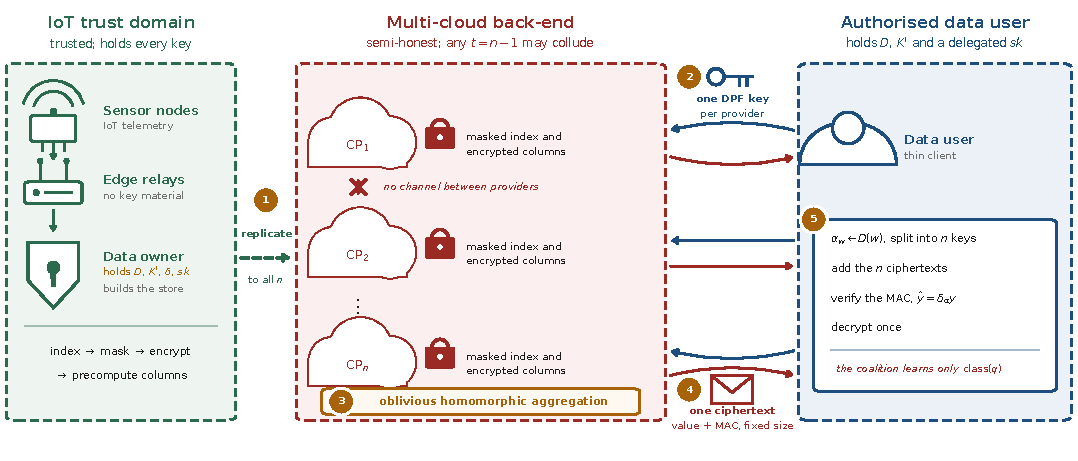
\includegraphics[width=\textwidth]{Figures/fig_architecture.pdf}
\caption{Overview of CR-SHE. The owner replicates a masked index and
encrypted columns to $n$ providers (1). A query is split into one DPF key per
provider (2), each provider aggregates obliviously over its own share (3) and
returns one ciphertext carrying value and MAC (4), and the user combines, verifies and decrypts
(5). No provider ever sees the matched set or its size.}
\label{fig:arch}
\end{figure*}

The adversary is probabilistic polynomial-time, static and semi-honest: it
fixes a coalition $C\subseteq[n]$ with $|C|\le t=n-1$, whose members follow
the protocol and pool everything they see, namely
\[
\mathrm{View}_C = \big( I',\ \text{CT},\ \widehat{\text{CT}},\ pk,\ pp,\
\{A_f,\widehat{A}_f\}_f,\ \{T_f,\widehat{T}_f\}_{f,\text{cube}},\
\{\kappa_{q,j},v_{q,j}\}_{j\in C,\,q\in[Q]} \big),
\]
plus the responses they compute, over adaptive queries. The goal is that this
view be simulatable from data-independent leakage revealing neither the
keyword or range, the access pattern, the result-set size, nor the result. The
DO and authorised DUs are honest, channels are authenticated and confidential,
and side channels beyond the message sizes accounted for here are out of scope.
Beyond this semi-honest goal we address two active threats. \emph{Deviating
providers} may return any response at all; the session check of
Section~\ref{sec:verify} makes every deviation that changes an answer evident
to the DU except with probability about $2^{-36}$ (Theorem~\ref{thm:tamper}),
without guaranteeing output delivery. \emph{Users exceeding their authority}
may send malformed keys or arbitrary share vectors; role-scoped columns and
mask keys confine a user to its own role's records
(Section~\ref{sec:auth}, Proposition~\ref{prop:role}). Collusion between a DU
and a provider is excluded, since a DU already holds decryption capability,
and a compromised DU exposes everything its role covers, since decryption is
delegated in full.

\section{The CR-SHE construction}
\label{sec:construction}

\subsection{Overview}
The DO builds a membership index $I\in\{0,1\}^{N\times N_d}$ in which keyword
$w$ occupies row $\alpha_w$ and $I[\alpha_w][i]=1$ if and only if record $i$
contains $w$. Rows are assigned by a secret, append-only dictionary $D$: a
keyword receives the next free row when it first appears and keeps it for the
lifetime of the deployment, so rows never move when keywords are added
(Section~\ref{sec:ingest}). The DO shares $D$ with authorised DUs and keeps it
from the providers, because the vocabulary itself, being device and site
names, is sensitive. Which row a keyword gets carries no security weight,
since providers see neither addresses nor unmasked rows; only injectivity
matters, for correctness. Rows are fixed width, so no row is distinguishable
by size, and the index is stored masked as $I'[x][i]=I[x][i]+P[x][i]\bmod p$
with $P$ drawn from the PRF $F'_{K'}$ by rejection sampling, so that every
entry is uniform on $\mathbb{Z}_p$ (Section~\ref{sec:mask}).
The computable field of each record is encrypted as
$\text{CT}_i=\Enc_{pk}(m_i)$, with a MAC column
$\widehat{\text{CT}}_i=\Enc_{pk}(\delta m_i)$; opaque payloads are encrypted
symmetrically.

A design that first recovers the selection vector at the client and then asks
the providers to evaluate $f$ over $\{\text{CT}_i\}_{i\in S}$ destroys in the
second step exactly what the first protected, because the providers are handed
$S$. CR-SHE therefore never materialises $S$ at a provider. Each provider
contracts its own share of the selection vector against the encrypted column
and returns one ciphertext. Algorithms~\ref{alg:outsource} and~\ref{alg:query}
summarise the owner outsourcing procedures and the per-query protocol.

\subsection{Why a homomorphic layer at $t=n-1$}
\label{sec:whyrep}
The obvious alternative to replicating ciphertexts is to deal the data to the
providers as an $(n,n)$ additive sharing over $\mathbb{Z}_p$ and answer DPF
queries over the shares, with no homomorphic encryption at all. Under our
constraints it does not work, and the reason fixes what any design here must
contain.

\begin{proposition}[No local answers over shares]
\label{prop:nolocal}
Let a column $A\in\mathbb{Z}_p^N$ be dealt as $A=\sum_{k\in[n]}S_k$, with
$S_1,\dots,S_{n-1}$ uniform and $\text{CP}_k$ holding $S_k$, and let $e_j$ be
the evaluation vector of DPF key $\kappa_j$ for $f_{\alpha,1}$. If each
provider returns $r_j=\langle e_j,S_j\rangle$, then
\[
\textstyle\sum_{j} r_j - A[\alpha] \;=\; -\sum_{j\neq k}\langle e_j,S_k\rangle ,
\]
and for $n=2$, whenever $e_1\neq e_2$, this error is uniform on
$\mathbb{Z}_p$ over the choice of $S_1$, so the answer is correct with
probability $1/p$; $e_1=e_2$ occurs only with negligible probability.
\end{proposition}
\begin{pf}
$A[\alpha]=\langle\sum_j e_j,\sum_k S_k\rangle=\sum_{j,k}\langle e_j,S_k\rangle$;
the providers' answers supply only the diagonal. For $n=2$, substituting
$S_2=A-S_1$ gives the error $-\langle e_1,A\rangle+\langle e_1-e_2,S_1\rangle$,
which is uniform because $S_1$ is uniform and independent of the keys, provided
$e_1\neq e_2$. Equality would mean $e_1=e_2=2^{-1}u_\alpha$; a provider could
test its own share for that form and read $\alpha$, so by $(n{-}1)$-privacy
equality has negligible probability. \qed
\end{pf}

The cross terms are not an artefact of choosing linear answers. Take any
non-interactive scheme in which $\text{CP}_1$ holds an additive share $S_1$ of
the data, the client forms its queries without reference to the data,
providers answer independently, and every query and response is shorter than a
share. Given a database $X$ held by a single server, a client
can run that scheme with $S_1:=X$ and the other shares drawn by itself, which
fixes the data as $A=X+\sum_{k>1}S_k$. It plays providers $2,\dots,n$ locally,
sends only the first query to the server, and subtracts $\sum_{k>1}S_k[\alpha]$
from the result. Privacy against the single provider $\text{CP}_1$ hides
$\alpha$ from the server, so this is a non-trivial single-server PIR scheme for
$X$, and such schemes imply oblivious transfer \citep{dicrescenzo2000single};
their standard instantiation is homomorphic encryption
\citep{kushilevitz1997replication}. Within that class, secret-sharing the data
does not remove the public-key primitive, it moves it into a per-share PIR; the
alternatives are interaction, for example multiplication triples, which the
no-channel constraint excludes, or assumptions outside the class, such as
preprocessing. The reduction does not show that every secret-sharing system
needs homomorphic encryption. The argument needs the
scheme to be correct on every tuple of shares, which holds for any scheme whose
answers are a deterministic function of the shares and the queries, and it
applies at $t=n-1$ with $(n,n)$ sharing. A lower threshold escapes it: with
$(t{+}1,n)$ threshold shares and $t<n/2$, providers can multiply two shared
values locally and the client interpolates the degree-$2t$ result, so
low-degree selection needs neither interaction nor a public-key primitive. That
appears to be the route of Shamir-shared systems such as Obscure
\citep{gupta2020obscure}, whose share multiplications raise the polynomial
degree and so the number of servers per tolerated colluder; we have not
verified its exact bound. A store replicated
under one owner's homomorphic key is the direct way to supply the primitive at
$t=n-1$, and it also brings three operational properties that a shared store
lacks.

\emph{Durability.} A sharing with privacy threshold $n-1$ is lost when any one
share is lost, whereas a replica set survives the loss of $n-1$ providers,
which is the reason multi-cloud deployments replicate at all. Threshold
sharing does not escape the trade-off: a $(t{+}1,n)$ scheme tolerates
$n-t-1$ losses, so at $t=n-1$ it degenerates to the $(n,n)$ case.

\emph{Graceful degradation.} A query needs every provider in the set it is
addressed to. With replicas, queries continue over any surviving set of at
least two providers, at that set's collusion bound, without touching stored
state; a shared store cannot answer until the dealer re-shares.

\emph{Key management and churn.} Encryption under one owner key lets the owner
rotate keys, revoke a provider, or add one by copying ciphertexts. Under
sharing, every change to the provider set re-deals the whole store, and the
dealer must hold the plaintext to do it.

\subsection{Oblivious homomorphic aggregation}
\label{sec:oha}
Suppose the providers hold additive shares $v_1,\dots,v_n\in\mathbb{Z}_p^{M}$
of a vector $v$ and replicas of an encrypted column
$\mathrm{C}=(\Enc_{pk}(c_1),\dots,\Enc_{pk}(c_M))$. Provider $j$ returns
\[
\text{ct}_j \;=\; \bplus_{i\in[M]} v_j[i]\bdot \mathrm{C}_i ,
\]
and the DU computes $\bplus_j \text{ct}_j$, which decrypts to
$\langle v,c\rangle$, and decrypts once. Nothing that leaves a provider depends
on $v$ beyond its own share, and the response is one ciphertext of fixed size
whatever the support of $v$. CR-SHE instantiates this contraction twice. On the
fast path (Section~\ref{sec:fast}) $v$ is the DPF's unit vector $u_{\alpha_w}$,
its shares are the evaluation vectors $e_j$, and $\mathrm{C}$ is a precomputed
aggregate column over the tag domain. On the flexible path
(Section~\ref{sec:flex}) $v$ is a selection vector over the records that the
client forms after a retrieval and deals as fresh shares, and $\mathrm{C}$ is
the record column. In both cases the matched set is never materialised at a
provider.

\begin{lemma}[Algebraic compatibility]
\label{lem:compat}
If the DPF output group and the HE plaintext ring are the same $\mathbb{Z}_p$,
and $\sum_{i}|w_f[i]\,m_i| < p$ for every admissible template, then for shares
$b_1,\dots,b_n\in\mathbb{Z}_p^{N_d}$ with $\sum_j b_j = \beta \bmod p$,
\begin{multline*}
\Dec_{sk}\Big(\bplus_{j\in[n]}\ \bplus_{i\in[N_d]}\ b_j[i]\bdot
\text{CT}_i\Big)\\
=\; \sum_{i\in[N_d]} \beta[i]\,m_i \pmod p .
\end{multline*}
\end{lemma}
\begin{pf}
$\bdot$ and $\bplus$ are homomorphisms over the same ring $\mathbb{Z}_p$, so
summation commutes with decryption and no reduction is lost: share addition
and plaintext addition are taken modulo the same modulus. The magnitude bound
prevents plaintext overflow. What remains is decryption correctness, which is
a noise-budget question rather than a depth question. A
plaintext-to-ciphertext product consumes no multiplicative level but scales
the noise by up to the norm of the plaintext, here as large as
$p\approx2^{36}$, because DPF shares are uniform in $\mathbb{Z}_p$, and the
contraction sums $\lceil N_d/\ell\rceil$ such products before a
rotate-and-sum. The parameters must leave room for that growth. We check the
worst case, full-magnitude coefficients across several packed chunks,
empirically rather than assume it (Section~\ref{sec:correctness}). \qed
\end{pf}

Lemma~\ref{lem:compat} is what makes the two primitives compose. Instantiating
the DPF over $\mathbb{Z}_{2^k}$ and the homomorphic scheme over an unrelated
plaintext modulus, which is the natural default since the two libraries are
chosen independently, silently breaks correctness through wraparound, and the
failure is data-dependent and therefore easy to miss in testing.

\subsection{Masking the index}
\label{sec:mask}
Retrieval (Section~\ref{sec:auth}) reads a row of the membership index through
the DPF. Stored in the clear, that index would hand every provider each
posting-list length, which the attack of Section~\ref{sec:leakeval} turns into
tag identities. As DORY does for its Bloom-filter bits \citep[\S4.1]{dory},
the DO therefore stores it one-time-padded, here with field-element masks so
that arithmetic DPF shares can strip them, and packed:
\[
I'[x][c]\;=\;\sum_{b<\pi} I[x][\pi c+b]\,2^b \;+\; P[x][c] \bmod p ,
\]
with $\pi=32$ membership bits per word, where row $P[x]$ is the output of
$F'_{K'}$ on $(x,\cdot)$ turned into exactly uniform elements of
$\mathbb{Z}_p$ by rejection sampling: each $64$-bit PRF word is cut to
$\lceil\log_2 p\rceil=37$ bits and kept only if it is below $p$, which accepts
a candidate with probability $p/2^{37}\approx0.5$. A packed word is below
$2^{32}<p$, so the pad still hides it perfectly, and the index occupies
$\lceil N_d/32\rceil$ words per row instead of $N_d$: a $32$-fold saving in
storage, in the retrieval pass and in its response. Because $p$ exceeds $2^{36}$,
the four spare bits double as a sanity check: a word at or above $2^{32}$ after
unmasking can only come from a corrupted share, and a uniformly corrupted word
passes with probability $1/16$. A retrieval returns shares of
$I'[\alpha_w]=\mathrm{pack}(b)+P[\alpha_w]$, and the DU, which derives
$P[\alpha_w]$ from $K'$, subtracts it and unpacks. No provider ever sees an
unmasked row or a mask value, and no correction ciphertext is needed.

\begin{theorem}[Index hiding]
\label{thm:mask}
For any two membership indexes $I_0,I_1\in\{0,1\}^{N\times N_d}$ packed $\pi$ bits per word into $\mathbb{Z}_p^{N\times\lceil N_d/\pi\rceil}$, no $\PPT$
distinguisher tells $\mathrm{pack}(I_0)+P$ from $\mathrm{pack}(I_1)+P$ with advantage greater than
$\advPRF_{F'}$. In particular the coalition learns no posting-list length, no
keyword-frequency multiset, and no membership relation from the stored index.
\end{theorem}
\begin{pf}
Replace $F'$ by a truly random function at the cost of $\advPRF$. A candidate
is then uniform on $\{0,\dots,2^{37}-1\}$, and conditioning on acceptance makes
each mask value exactly uniform on $\mathbb{Z}_p$, independently of every
other. $\mathrm{pack}(I_b)+P$ is then a one-time pad of $\mathrm{pack}(I_b)$ and is uniform on
$\mathbb{Z}_p^{N\times\lceil N_d/\pi\rceil}$ for either $b$. \qed
\end{pf}

Reducing uniform $64$-bit words modulo $p$ instead, as is common, biases each
mask word: with $r=2^{64}\bmod p$ its statistical distance from uniform is
$r(p-r)/(p\,2^{64})\approx8.27\times10^{-10}$ for our modulus. Over the
$N\lceil N_d/32\rceil=146{,}625{,}960$ words of the packed telemetry index the
union bound is about $0.12$, and over the $NN_d$ words of an unpacked index it
exceeds $1$ and says nothing. These are upper bounds, not measured
distinguishing advantages, but they make rejection sampling, at about two PRF
words per mask value, necessary for Theorem~\ref{thm:mask} to hold as stated.
\authorcheck{The C++ prototype still reduces 64-bit words over an unpacked
index, so Theorem~\ref{thm:mask} does not cover the index its leakage
experiment used; port the rejection sampler of crshe/prg.py and re-run
Section~\ref{sec:leakeval}.}

\begin{remark}[Stripping the mask first]
\label{rem:whyenc}
An alternative contracts the masked shares $b_j$ directly against the record
column and cancels the resulting term
$u_f(\alpha_w)=\sum_i w_f[i]\,P[\alpha_w][i]\,m_i$ with an encrypted correction
column $U_f=(\Enc_{pk}(u_f(x)))_{x\in[N]}$, retrieved by the same DPF. An
earlier version of our design did this. It has two defects. $U_f$ must be precomputed by
the DO for each weight vector, so it serves only registered weights, for which
the fast path is cheaper; it cannot serve the ad-hoc weights and conjunctions
it was meant for. And the correction must itself be encrypted: published in the
clear, the count correction $g(x)=\sum_iP[x][i]$ gives
$\sum_iI'[x][i]-g(x)=|I[x]|$, the row Hamming weight, restoring the volume
leakage the mask removes. The flexible path avoids both by stripping the mask
at the client before any contraction.
\end{remark}

\subsection{Precomputed columns: the single-keyword fast path}
\label{sec:fast}
The contraction of Section~\ref{sec:oha} costs $\Theta(N N_d)$ ring operations
per provider per query, which is the price of hiding the access pattern
without preprocessing, by the lower bounds underlying ORAM and PIR
\citep{goldreich1996software,beimel2000reducing}. For the common case, an
aggregate over the whole posting list of a single keyword under a template
registered at setup, this cost is avoidable. The DO precomputes, for every
$x\in[N]$,
\[
A_f[x] \;=\; \sum_{i\in[N_d]} I[x][i]\,w_f[i]\,m_i \bmod p ,
\]
and publishes it as $\lceil N/\ell\rceil$ packed ciphertexts. A query then
reduces to an oblivious retrieval of one element of an encrypted length-$N$
array:
\[
\text{ct}_j \;=\; \bplus_{x\in[N]} e_j[x]\bdot A_f[x],
\]
costing $O(N)$ pseudorandom-generator calls for the full-domain evaluation
plus $O(N/\ell)$ packed ciphertext-plaintext multiplications and
$O(\log \ell)$ rotations, \emph{independent of $N_d$}. No mask correction is
needed on this path, because $A_f$ is derived from the unmasked $I$ held by
the DO and is itself encrypted.

The fast path supports the templates registered at setup, namely count, sum,
per-sensor-band sums, and fixed plaintext-weighted inner products, applied to
a single keyword. Conjunctive queries and ad-hoc weight vectors chosen at
query time use the flexible path of Section~\ref{sec:flex}. Insertion is
cheap: a new record carrying $\tau$ tags updates $A_f$ at $\tau$ addresses in
plaintext at the DO, followed by re-encryption of all of the column's packed
ciphertexts, for the reason given in Section~\ref{sec:ingest}; no decryption
is involved.

\subsection{Packing the response}
\label{sec:packing}
The straightforward layout spends two ciphertexts on one scalar: the value and its MAC
(Section~\ref{sec:verify}), each column packed across all $\ell$ slots and
summed over all of them, so that $\ell-1$ slots of each response go unused.
BFV slots have more structure than that. With ring dimension $\ell$ they form
two rows of $\ell/2$, and the automorphisms behind rotation act within each row
\citep{halevi2014algorithms}. CR-SHE uses that shape directly. The DO packs
$A_f$ in row~$0$ and $\widehat{A}_f$ in row~$1$, chunked $\ell/2$ tags per
ciphertext; the provider multiplies each chunk by its evaluation vector,
replicated in both rows, adds the chunks, and rotates and sums within the rows.
Slot~$0$ then carries the value share and slot~$\ell/2$ the MAC share, in one
ciphertext.

Several templates share that ciphertext. For $k$ templates, $k$ a power of
two, each row is cut into $k$ segments of $s=\ell/(2k)$ slots, template $r$
occupying segment $r$ of both rows, with $\lceil N/s\rceil$ chunks. Rotating
and summing by $1,2,\dots,s/2$ leaves the sum of segment $r$ in its first slot,
so slot $rs$ of each row carries template $r$'s value or MAC share.
Explicitly, chunk $c$ holds, at offset $z<s$ of segment $r$,
\[
\text{row }0:\ A_{f_r}[cs+z],\qquad
\text{row }1:\ \begin{cases}A_{f_r}[cs+z] & \text{session check},\\
\delta_{cs+z}\,A_{f_r}[cs+z] & \text{per-row keys},\end{cases}
\]
zero beyond $N$, and the provider's plaintext for chunk $c$ repeats its
evaluation share $e_j[cs+z]$ in every segment of row~$0$ and the
$\delta_s$-carrying share $\hat e_j[cs+z]$ in every segment of row~$1$. The
response is one ciphertext for any $k\le\ell/2$; what grows with $k$ is the
number of chunks, $\lceil kN/(\ell/2)\rceil$ plaintext-ciphertext products,
while the rotations fall from $\log_2(\ell/2)$ to $\log_2 s$. The worked
instance of a \textsc{mean} below needs its count and sum in one response;
count, sum and sum of squares give a variance in one round.

Finally, the provider drops the response to a single RNS tower by modulus
switching before it sends it. At multiplicative depth one, decryption is
unaffected, and the ciphertext halves. Against the two-ciphertext layout, which
costs $2\lceil N/\ell\rceil$ products and $2\log_2\ell$ rotations per template,
packing halves the provider's homomorphic work (rotations dominate at these
parameters) and quarters the downlink, and for four templates cuts the
downlink sixteen-fold (Section~\ref{sec:packresult}). The natural single-server
alternative, one server answering the same query over the same encrypted
columns, uses this same layout with an encrypted one-hot
query in place of the DPF shares; Section~\ref{sec:packresult} measures it.

\subsection{Oblivious range aggregation over data cubes}
\label{sec:range}
A single tag answers a narrow question: the mean over one minute, one site, or
one value band. The questions IoT analysts ask are ranges, such as the mean
temperature at one device over an afternoon, or the number of hours in which a
pollutant sat in its top three bands. Composing such a query from single-tag
aggregates costs one query per tag in the range and reveals its length, and the
flexible path costs a retrieval per tag. CR-SHE answers rectangular ranges in
one round, at a cost independent of both the range and the record count.

\emph{Data cubes.} The DO registers a \emph{data cube}: $d$ ordered tag
families $\mathcal{F}_1,\dots,\mathcal{F}_d$ of sizes $s_1,\dots,s_d$, for
example device, one-minute window and the decile band of one sensor, such that
every record $i$ falls in exactly one cell $c(i)\in\prod_k[s_k]$. For each
registered template $f$ the cell aggregate is
$C_f[c]=\sum_{i:\,c(i)=c}w_f[i]\,m_i$, and the DO stores the $d$-dimensional
prefix sums, the summed-area table
\[
T_f[c] \;=\; \sum_{c'\le c} C_f[c'] ,
\]
with $\le$ taken coordinate-wise, flattened row-major into a column of
$M=\prod_k s_k$ entries and packed like a fast-path column
(Section~\ref{sec:packing}). Prefix-sum cubes are a classical OLAP structure;
what is new here is answering them obliviously over encrypted replicas.

\emph{Queries.} For a box $B=\prod_k[\mathit{lo}_k,\mathit{hi}_k]$ and
$\sigma\in\{0,1\}^d$, let corner $\kappa_\sigma(B)$ take $\mathit{lo}_k-1$ on
the axes where $\sigma_k=1$ and $\mathit{hi}_k$ elsewhere. By
inclusion--exclusion,
\begin{equation}
\label{eq:ie}
\sum_{c\in B} C_f[c] \;=\; \sum_{\sigma\in\{0,1\}^d} (-1)^{|\sigma|}\,
T_f[\kappa_\sigma(B)],
\end{equation}
where a corner with a coordinate equal to $-1$ lies outside the cube and
contributes $0$. The DU sends, for every $\sigma$, one DPF key per provider
for the point function at $\kappa_\sigma(B)$ with output
$\beta_\sigma=(-1)^{|\sigma|}\bmod p$. For a corner outside the cube it sends a
\emph{dummy} key, with $\beta_\sigma=0$ at a uniformly random point. DPF keys
hide $\beta$ as well as the point, so every query to a cube carries exactly
$2^d$ indistinguishable keys per provider, and a provider cannot tell a range
that starts at the cube's edge from one in its interior.

\emph{Answering.} Provider $j$ evaluates its $2^d$ keys over the full domain of
$M$ cells, adds them, $e_j=\sum_\sigma e_{\sigma,j}$, and contracts once against
the encrypted table; the response is one ciphertext. The DU adds the $n$
responses and decrypts, and slot $0$ holds the range aggregate. In the
\emph{verified} layout, row~$1$ of the table is a copy of row~$0$ and the query
carries a second set of $2^d$ keys with outputs $\delta_s\beta_\sigma$; the
provider places $\hat e_j=\sum_\sigma\hat e_{\sigma,j}$ in row~$1$ of the same
plaintexts, so slot $\ell/2$ holds $\delta_s$ times the aggregate
(Section~\ref{sec:verify}). An earlier \emph{per-corner} layout instead gave
each corner its own slot segment, checked against a per-cell MAC key; it stores
the table $2^d$ times and misses deviations at the queried corner, and we keep
it only as a measured baseline.

\emph{Cost.} Per provider: $2^d$ full-domain DPF evaluations over $M$ cells
($2^{d+1}$ in the verified layout), $\lceil kM/(\ell/2)\rceil$
plaintext-ciphertext products for $k=|\{f\}|$ templates, and
$\log_2(\ell/2k)$ rotations. Uplink is $2^d$ two-party keys of
$O(\lambda\log M)$ bits each, or $2^{d+1}$ verified. Nothing depends on the box
or on $N_d$.

\emph{Magnitude and updates.} Every table entry is at most the cube's total,
so Lemma~\ref{lem:compat} requires $\sum_i w_f[i]m_i<p$ over the whole corpus,
a stronger condition than for a single tag. With time as the outermost axis
and no later slices yet, a batch of records appended to the newest time slice
changes $T_f$ only in that slice, so the DO would re-encrypt only the
ciphertexts covering it, and since time advances publicly the write pattern
would reveal nothing new. When whole-cube replacement is used instead, the
update leakage matches that of the fast-path columns in
Section~\ref{sec:ingest}. We have not implemented or measured either update,
and their write patterns belong in an update-leakage analysis we have not done.
Role-scoped tables (Section~\ref{sec:auth}) multiply storage by the number of
roles.

\emph{Why prefix sums rather than interval FSS.} Boyle, Gilboa and Ishai
give FSS for $d$-dimensional intervals with key size $O(\lambda n^d)$, built by
the same inclusion--exclusion over $2^d$ zero-anchored intervals, each shared
as a decision tree \citep[\S3.3, Cor.~3.4]{boyle2016function}. Evaluating such
keys requires the servers to hold each record's coordinates, as Splinter's
providers hold public data \citep{splinter}; over owner-encrypted records the
coordinates themselves (which device, which minute, which band) are the
sensitive part. Moving the prefix sums into a dense, encrypted table over all
$M$ cells keeps the coordinates hidden, reveals only the cube's dimensions, and
lets each of the $2^d$ pieces be a point function with a key of
$O(\lambda\log M)$ bits. The price is that cubes and templates must be
registered and precomputed, and that cost grows with $M$ rather than with the
number of records.


\subsection{Tamper evidence}
\label{sec:verify}
Every response carries a second slot row (Section~\ref{sec:packing}), so a
check value travels with the answer at no extra downlink. Three ways to fill
that row differ in what they catch.

\emph{One owner key.} Row~$1$ holds $\delta m_i$, or $\delta A_f[x]$, under a
single secret $\delta$, and the DU accepts only if $\hat y=\delta y$. A provider
that adds a constant, corrupts one half, or returns a stale or foreign
ciphertext is caught except with probability $1/p$. One that applies the
\emph{same} linear substitution to both halves passes: contracting against any
$e'_j$ instead of $e_j$, for instance $k\,e_j$, shifts $y$ and $\hat y$ by
amounts in the ratio $\delta$, so the tag still verifies.

\emph{Per-position keys.} Row~$1$ holds $\delta_xA_f[x]$ with
$\delta_x=F''_{K''}(x)$, or $\delta_cT_f[c]$ per cube cell, and the DU checks
against the key of the queried position. A substitution $e_j+d$ then passes
only if $\sum_{x\neq\alpha_w}d[x](\delta_x-\delta_{\alpha_w})A_f[x]=0$, a
non-zero linear form in independent keys whenever $d$ touches a non-empty
position other than $\alpha_w$. What survives is a deviation concentrated on
the queried position itself, which rescales the answer; a provider that guesses
or knows that position wins. Per-position keys also do not exist for the
flexible path, whose contraction runs over records.

\emph{A per-query secret.} The session layout stores no key at all: row~$1$ of
every column, aggregate column or table is a copy of row~$0$. With each query
the DU draws a fresh $\delta_s$ uniformly from $\mathbb{Z}_p^{*}$ and sends a
second set of keys for the same points with outputs multiplied by $\delta_s$:
$f_{\alpha_w,\delta_s}$ on the fast path, $\delta_s\beta_\sigma$ at each corner
of a range, and fresh shares of $\delta_s v$ in a flexible round. Each provider
places the second evaluation vector in row~$1$ of the same plaintexts, so the
homomorphic work is unchanged and slot $\ell/2$ decrypts to $\delta_s y$. The
DU accepts only if $\hat y=\delta_s y$.

\begin{theorem}[Tamper evidence]
\label{thm:tamper}
Consider one query in the session layout on any path. Let a coalition $C$ of at
most $n-1$ providers return arbitrary responses computed from its members'
views, with at least one honest provider, an honest DU that keeps $\delta_s$
secret, and no provider colluding with the DU; the coalition does not see the
honest providers' keys, and the DU decrypts whatever ciphertexts it receives.
Let $y$ be the honest answer. The DU accepts an output $y'\neq y$ with probability at most
\[
\frac{1}{p-1}+\varepsilon,
\]
where $\varepsilon=\kappa\,\advDPF$ for a query whose $\delta_s$-carrying set
has $\kappa$ DPF keys per provider ($\kappa=1$ on the fast path and for a
retrieval, $2^d$ for a range) and $\varepsilon=\advPRF$ for a flexible round. Over $Q$ queries the
bounds add, whether or not the coalition learns which queries were accepted.
\end{theorem}
\begin{pf}
Let $V$ be the coalition's view: both key sets of its members, the stored
ciphertexts, the public and evaluation keys, and everything it saw in earlier
queries. Its responses decrypt, summed over $C$, to $(r_0,r_1)$ in the slots of
one template, a function of $V$, the database and the coalition's coins; the
decryption key is independent of $\delta_s$. Let $y_C$ and $\hat y_C$ be what
the members of $C$ would have contributed honestly, also functions of $V$ and
the database. The honest providers contribute $y-y_C$ and
$\delta_sy-\hat y_C$, so the DU decrypts $y'=y-y_C+r_0$ and
$\hat y'=\delta_sy-\hat y_C+r_1$ and accepts if and only if
\[
r_1-\hat y_C=\delta_s\,(y'-y).
\]
Replace the coalition's $\delta_s$-carrying keys by keys for the same points
and an independent scalar $\delta'_s$. A reduction that knows the points, the
signs, the database and $\delta_s$ can evaluate the event
$\{y'\neq y\wedge r_1-\hat y_C=\delta_s(y'-y)\}$ from the coalition's keys and
outputs, so by $(n{-}1)$-privacy, which hides the output $\beta$ as well as the
point, its probability changes by at most $\kappa\,\advDPF$; for a flexible
round the coalition's shares of $\delta_sv$ are uniform, or pseudorandom when a
seed is missing, at cost $\advPRF$. After the change $V$ is independent of
$\delta_s$. Conditioned on $V$, the database and the coins, everything in the
displayed equation except $\delta_s$ is fixed, and since $y'-y\neq0$ at most one
of the $p-1$ equally likely values of $\delta_s$ satisfies it. Each query uses
a fresh $\delta_s$, so feedback from earlier queries concerns independent
scalars, and a union bound over the $Q$ queries completes the proof. \qed
\end{pf}

The bound needs no restriction on how a provider deviates: it may substitute
vectors, rescale the queried point, swap or mix slot rows, replay an old
response or return any ciphertext at all. It does not guarantee output
delivery, since a deviating provider can always force an abort. It also leaves
one channel open: whether the DU aborts can depend on the data, for example on
whether a cell a provider chose to perturb is empty, so a DU that reveals its
aborts can leak up to one bit about the data per query to a malicious
provider, though nothing about the query, whose keys are pseudorandom to it. A
DU that retries silently through another provider set closes that channel.
The $200$ injected trials per deviation in Section~\ref{sec:verifyresult} are
empirical checks of the implementation, not a measurement of the $1/(p-1)$
bound.\authorcheck{Have the session-check reduction, including the
computational DPF hybrid and adaptive abort leakage, checked by a reader outside
the project.}
Against per-position keys the cost is a second key set and a second full-domain
evaluation per provider, with no extra homomorphic product and no stored key;
Section~\ref{sec:verifyresult} measures all three modes on every path.

\subsection{Record retrieval and role-scoped access}
\label{sec:auth}
When the DU needs payloads, providers return $b_j$ directly; the DU subtracts
$P[\alpha_w]$, unpacks $b$, and fetches the payloads with a batch of
$k_{\max}$ DPF retrievals padded to a public bound, as in Splinter
\citep{splinter}. The response is $\lceil N_d/32\rceil$ words whatever $|S|$.

\emph{Why providers cannot check a query.} DPF privacy hides the queried row,
so no provider can check \emph{which} keyword, cell or range a query targets.
Keys that are not point functions (an $n$-party key \emph{is} a share vector,
and a two-party key is pseudorandom) give arbitrary linear combinations of
rows, columns or cells, and the flexible path's second round is by
construction an oracle for any linear function of the record column. A user
with query access can therefore read everything its columns and mask key
cover. Proofs carried with the key \citep{pacl,ji2023finegrained} or verifiable
DPFs \citep{decastro2022lightweight} restrict which keys are accepted, at the
price of a short server-to-server exchange in the constructions we know
\citep{boneh2021lightweight}. We restrict instead what the columns and keys
cover.

\emph{Role-scoped columns and keys.} The DO assigns every record a role
$\rho(i)\in[R]$, for example the agency that owns the device, and lays out
record identifiers so that each packed word of the index holds records of one
role, padding with empty records where a role's records end. It derives one
mask key per role, $K'_\rho=F_{K'}(\rho)$, and draws word $c$ of every index row
from $K'_{\rho(c)}$; a user of role $\rho$ receives $K'_\rho$ only. For every
role the DO also builds the aggregate columns $A_f^{\rho}$, the cube tables
$T_f^{\rho}$ and the record column from that role's records alone, zero
elsewhere. A provider answers a role-$\rho$ user from role $\rho$'s columns,
selected by the user's authenticated identity; that policy lookup is the only
role-dependent provider logic, and it needs no exchange with other providers.

\begin{proposition}[Role confinement]
\label{prop:role}
Suppose every provider authenticates the data user's role and applies that
role's columns on every response path, and no provider colludes with the data
user. Then for any sequence of queries a role-$\rho$ user sends,
including malformed keys and arbitrary share vectors, its view is simulatable
from the role-$\rho$ records and the public dimensions, up to
$\advPRF$.
\end{proposition}
\begin{pf}
Fast-path, range and flexible responses are linear functions of the
role-$\rho$ columns, which are functions of role-$\rho$ records only. A
retrieval returns linear combinations of masked index entries. Entries in
role-$\rho$ words depend on role-$\rho$ records and on masks the user can
derive. Entries in other words carry masks from keys $K'_{\rho'}$,
$\rho'\neq\rho$, which the user lacks; replacing $F$ by a random function at
cost $\advPRF$ makes those masks one-time pads, so the entries are uniform
whatever the records. \qed
\end{pf}

The mechanism costs storage, not interaction: columns, tables and record
columns are replicated per role, while the large masked index is shared. It
reveals each query's role to the providers and each role's size, rounded up to
a word, in the public layout. Confinement is conditional on provider-side
enforcement: a provider that colludes with an unauthorised user defeats it. It
does not express policies finer than a record
partition, such as per-tag rights within a role; revoking a user of a role
means re-keying that role and re-masking its words; and a streaming deployment
must keep one hot buffer per role, so that every packed word stays within one
role.

\subsection{The flexible path: conjunctions and ad-hoc weights}
\label{sec:flex}
Registered single-keyword templates cover the common case. For anything else,
such as a conjunction or disjunction of keywords, a weight vector chosen at
query time, or a threshold on the matched set, the DU runs two rounds.

\emph{Round one} is a retrieval (Section~\ref{sec:auth}) for each keyword
involved, after which the DU holds the posting lists and forms whatever
selection vector it needs over the records, for example
$v=w\circ(b_{w_1}\wedge b_{w_2})$ for an ad-hoc weight vector $w$ and a
conjunction of two keywords.

\emph{Round two} deals $v$ as fresh additive shares $v=\sum_jv_j$ over
$\mathbb{Z}_p$, compressed exactly like the $n$-party key of
Section~\ref{sec:prelim}: $n-1$ providers receive a $\lambda$-bit seed whose
PRF expansion is their share, and one receives the explicit difference vector.
Each provider runs the contraction of Section~\ref{sec:oha} against the record
column, packed with $m_i$ in row~$0$ and $m_i$ (session check, with shares of $\delta_s v$ in row~$1$) or $\delta m_i$ (stored key) in row~$1$ of
$\lceil N_d/(\ell/2)\rceil$ ciphertexts, and returns one ciphertext. The DU
adds the $n$ responses, decrypts once and checks $\hat y=\delta_s y$ (session) or $\delta y$ (stored key). The
magnitude bound of Lemma~\ref{lem:compat} is the DU's to check, against a
public bound on $m_i$, since it alone knows $v$.

Round two costs $\lceil N_d/(\ell/2)\rceil$ plaintext-ciphertext products and
$\log_2(\ell/2)$ rotations per provider, $\lambda$ bits of uplink to $n-1$
providers and $N_d\lceil\log p\rceil$ bits to one, and one ciphertext down.
Every share a coalition of $n-1$ providers holds is uniform, or pseudorandom
for the seeds, independently of $v$, so round two adds to the coalition's view
nothing that depends on the query (Theorem~\ref{thm:sec}). The DU learns $S$
and $|S|$, which $\Leak^{\text{DU}}$ already contains.

A single round is not possible here in general: a conjunction is the product
of two selection vectors, which no linear contraction of shares computes, and
an ad-hoc weight vector would need a mask correction the DO cannot precompute
(Remark~\ref{rem:whyenc}).

\subsection{Dynamic ingest}
\label{sec:ingest}
IoT streams are append-only. CR-SHE keeps a static tier and a hot buffer of at
most $B$ records scanned by the same contraction, folded into a rebuilt tier
every $B$ insertions. Because the coalition's per-query view is independent of
the query (Theorem~\ref{thm:sec}), a query reveals nothing about records
inserted before or after it, which is forward and backward privacy in the usual
sense; what updates themselves expose is the public tier metadata in the setup
leakage, and we do not analyse update leakage beyond that.
Three rules keep updates from leaking. \emph{Rows never move}: a new keyword
takes the next free, masked, all-zero row of $D$, so only exhausting the
provisioned headroom is visible. \emph{A fresh mask key per static tier}: a
rebuild re-lays the record axis, and reusing $K'$ would expose the change in
membership. \emph{Whole columns are replaced}: re-encrypting only the affected
ciphertexts of $A_f$ would reveal which blocks of tags changed; summed-area
tables with time as the outermost axis would be the exception
(Section~\ref{sec:range}), since only the newest, publicly known slice changes.
The C++ prototype implements and measures the hot buffer and the fast-path
rebuild (Section~\ref{sec:setupresult}); the reference implementation does
not, and neither implements the summed-area-table update.

\begin{algorithm}[t]
\footnotesize
\caption{Outsourcing at the data owner.}
\label{alg:outsource}
\begin{algorithmic}[1]
\Procedure{$\mathsf{Setup}$}{$1^\lambda,n,t,p$}
  \State $D\gets\emptyset$; \ $K',K''\gets\{0,1\}^\lambda$; \
         $\delta\gets\mathbb{Z}_p^{*}$
  \State $(pk,sk)\gets\mathsf{KGen}(1^\lambda,L_{\mathrm{HE}},p,\ell)$
  \State $pp\gets(n,t,N,N_d,p,\ell,\{w_f\})$
  \State \Return $(D,K',\delta,pk,sk,pp)$
\EndProcedure
\Statex
\Procedure{$\mathsf{BuildIndex}$}{$D,K',DB$}
  \State $D(w)\gets|D|$ for each new $w$
         \Comment{rows never move}
  \State $I[D(w)][i]\gets 1$ for each keyword $w$ of record $i$
  \State $P[x]\gets$ rejection-sampled $F'_{K'}(x,\cdot)$
  \Statex \hfill uniform on $\mathbb{Z}_p^{\lceil N_d/\pi\rceil}$, for all $x\in[N]$
  \State $I'\gets \mathrm{pack}(I)+P \bmod p$
  \State \Return $I'$ \Comment{replicated to all $\text{CP}_j$}
\EndProcedure
\Statex
\Procedure{$\mathsf{Precompute}$}{$pk,K',DB,\{w_f\}$}
  \ForAll{registered templates $f$}
    \State $A_f[x]\gets\sum_i I[x][i]\,w_f[i]\,m_i$
    \State $\widehat{A}_f[x]\gets\delta_x A_f[x]$,
           \ $\delta_x\gets F''_{K''}(x)$
    \State pack $A_f$ in row 0, $\widehat{A}_f$ in row 1,
    \Statex \hfill templates in segments (\S\ref{sec:packing}); encrypt
  \EndFor
\EndProcedure
\Statex
\Procedure{$\mathsf{EncData}$}{$pk,DB$}
  \State pack $m_i$ in row 0, $\delta m_i$ in row 1; encrypt
  \Statex \hfill $\lceil N_d/(\ell/2)\rceil$ ciphertexts
  \State symmetric-encrypt opaque payloads
\EndProcedure
\end{algorithmic}
\end{algorithm}

\begin{algorithm}[t]
\footnotesize
\caption{Query, at the data user and at provider $\text{CP}_j$.}
\label{alg:query}
\begin{algorithmic}[1]
\Procedure{$\mathsf{Token}$}{$D,w,f$}
  \Comment{at the DU}
  \State $\alpha_w\gets D(w)$
  \State $(\kappa_1,\dots,\kappa_n)\gets\Gen(1^\lambda,\alpha_w,1)$
         over $\mathbb{Z}_p$
  \State verified: $\delta_s\gets\mathbb{Z}_p^{*}$;
         $(\hat\kappa_1,\dots,\hat\kappa_n)\gets\Gen(1^\lambda,\alpha_w,\delta_s)$
  \State \Return $(\kappa_j,\hat\kappa_j,f)\to\text{CP}_j$
\EndProcedure
\Statex
\Procedure{$\mathsf{FastAgg}$}{$\kappa_j,\hat\kappa_j,f,A_f,\widehat{A}_f$}
  \Comment{single keyword (Algorithm~\ref{alg:outsource} columns)}
  \State check the shape of $\kappa_j,\hat\kappa_j$
         \Comment{\S\ref{sec:auth}}
  \State $e_j[x]\gets\Eval(j,\kappa_j,x)$; \ $\hat e_j[x]\gets\Eval(j,\hat\kappa_j,x)$, $x\in[N]$
         \Comment{$O(N)$ PRG}
  \State $\text{ct}_j\gets\bplus_{c} E_{j,c}\bdot \mathrm{A}_c$
         \Comment{$O(N/\ell)$ HE}
  \Statex \hfill $E_{j,c}$: chunk $c$ of $e_j$ in row 0, $\hat e_j$ (or $e_j$) in row 1
  \State rotate and sum within segments; compress
  \State \Return $\text{ct}_j$
         \Comment{one ct, value + MAC}
\EndProcedure
\Statex
\Procedure{$\mathsf{Deal}$}{$v,\delta_s$}
  \Comment{at the DU, flexible}
  \State $v=\sum_j v_j$, $\delta_s v=\sum_j \hat v_j$: seeds to $n-1$ providers,
  \Statex \hfill explicit difference to one
\EndProcedure
\Statex
\Procedure{$\mathsf{FlexAgg}$}{$v_j,\hat v_j,\text{CT}$}
  \Comment{round two ($V_{j,c}$: $v_j$ in row 0, $\hat v_j$ or $v_j$ in row 1)}
  \State $\text{ct}_j\gets\bplus_c V_{j,c}\bdot\text{CT}_c$;
         rotate and sum
  \State \Return $\text{ct}_j$
\EndProcedure
\Statex
\Procedure{$\mathsf{Retrieve}$}{$\kappa_j,I'$}
  \State \Return $b_j\gets\sum_{x} e_j[x]\cdot I'[x]$
         \Comment{fixed size}
\EndProcedure
\Statex
\Procedure{$\mathsf{CombineDec}$}{$sk,K',\delta,\cdot$}
  \Comment{at the DU}
  \State $(y,\hat y)\gets$ slots $(0,\ell/2)$ of
         $\Dec(sk,\bplus_j\text{ct}_j)$
  \State \textbf{abort} if $\hat{y}\neq\delta_s y$ (session), or
         $\delta_{\alpha_w}y$, $\delta y$ (stored keys)
  \State retrieval: $b\gets\mathrm{unpack}\big((\sum_j b_j)-P[\alpha_w]\big)$
  \State \hskip2em $S\gets\{i: b[i]=1\}$
  \State \Return $y$, and $S$ if retrieving
\EndProcedure
\end{algorithmic}
\end{algorithm}

\subsection{Worked instance}
A clinician queries the tag \texttt{arrhythmia} with the registered template
\textsc{mean}. The DU derives $\alpha_w$ and sends one DPF key per provider.
Each provider performs a full-domain pass, contracts against the
\textsc{sum} and \textsc{count} columns packed side by side, and returns one
ciphertext carrying both values and both MACs. The DU adds the shares,
decrypts once, verifies the MACs, and divides. No provider, and no coalition of up to $n-1$, learns the tag
queried, which records contributed, how many did, or the mean itself.

% ===========================================================================
\section{Security analysis}
\label{sec:security}

\emph{Leakage profile.} We define
$\Leak=(\Leak_{\mathrm{Setup}},\Leak^{\text{CP}},\Leak^{\text{DU}})$ with an
observer split:
\begin{align*}
\Leak_{\mathrm{Setup}}(DB) &= (n,t,N,N_d,p,\ell,\mathrm{layoutMeta},\mathrm{cubeMeta},\mathrm{roleMeta},\mathrm{tierMeta}),\\
\Leak^{\text{CP}}_{\mathrm{Query}} &= \mathrm{class}(q),\\
\Leak^{\text{DU}}_{\mathrm{Query}} &= \big(|S|,\ f(\mathrm{records}(S))\big).
\end{align*}
The setup leakage is everything a provider can see in its replica:
$\mathrm{layoutMeta}$ gives the registered templates and the segment and
ciphertext-column shapes, $\mathrm{cubeMeta}$ the registered cubes and their
dimensions $(s_1,\dots,s_d)$, $\mathrm{roleMeta}$ the number of roles and each
role's span of packed words, and $\mathrm{tierMeta}$ the tier sizes and epochs.
Here $\mathrm{class}(q)$ says whether a query is a fast-path aggregate over a
named layout of registered templates, a range aggregate over a named cube and
layout, a retrieval, or the second round of a flexible query, together with
the querying user's role and whether the query carries the verification key
set. The coalition
learns that and the public dimensions of the deployment, and nothing else: not
the keyword, not the range or whether it touches the cube's edge, not the
access pattern, not $|S|$, not the weights, not the result. In contrast to a design in which
the matched set is returned to the providers for evaluation, and in contrast
to an unmasked index, $\Leak_{\mathrm{Setup}}$ here contains no posting-list
lengths and no membership structure, by Theorem~\ref{thm:mask}. Retrieval adds
the public padding bound $k_{\max}$ to $\Leak^{\text{CP}}$. A conjunctive
query is two retrievals and one flexible round, adding only result sizes to
$\Leak^{\text{DU}}$, never to the coalition.

\begin{definition}[$\Leak$-security against $t$-collusion]
\label{def:sec}
In $\Real_{\Adv,\Pi}(1^\lambda)$: (1) $\Adv$ outputs $(DB,C)$ with $|C|\le t$;
(2) the challenger runs $\mathsf{Setup}$, $\mathsf{BuildIndex}$,
$\mathsf{Precompute}$, $\mathsf{EncData}$ and gives $\Adv$ the static view
$(I',\text{CT},\widehat{\text{CT}},\{A_f,\widehat A_f\}_f,\{T_f,\widehat
T_f\}_{f,\text{cube}},pk,pp)$;
(3) for $q=1,\dots,Q$, $\Adv$ adaptively issues a query (a keyword with a
template layout, a box of a registered cube with a layout, a keyword to
retrieve, or a selection vector $v_q$ for a flexible round) and receives the coalition's per-query view: its DPF keys
$\{\kappa_{q,j}\}_{j\in C}$ or its shares $\{v_{q,j}\}_{j\in C}$, including the
$\delta_s$-carrying set of a verified query, and the responses those providers
compute; (4) $\Adv$
outputs a bit. In $\Ideal_{\Adv,\Sim,\Leak}(1^\lambda)$ a $\PPT$ simulator
$\Sim$ produces the views given only $\Leak_{\mathrm{Setup}}$ and the
per-query leakage. $\Pi$ is $\Leak$-adaptively-secure against $t$-collusion if
for every $\PPT$ $\Adv$ corrupting $\le t$ providers there is a $\PPT$ $\Sim$
with $|\Pr[\Real=1]-\Pr[\Ideal=1]|\le\negl(\lambda)$.
\end{definition}

\begin{theorem}[Correctness]
\label{thm:correct}
Fix a database $DB$, a keyword $w$, and a registered template $f$ satisfying
the magnitude bound of Lemma~\ref{lem:compat}. Then $\mathsf{CombineDec}$
returns $y=\sum_{i\in S} w_f[i]\,m_i$ with $S=\{i: I[\alpha_w][i]=1\}$ on the
fast path, a range query on a box $B$ of a registered cube whose total is
below $p$ returns $\sum_{i:\,c(i)\in B}w_f[i]\,m_i$, $\mathsf{Retrieve}$
returns exactly $S$, and a flexible round on a selection vector $v$ satisfying
the magnitude bound returns $\sum_i v[i]\,m_i$, except with the negligible
probability that leveled-HE decryption fails.
\end{theorem}
\begin{pf}
By DPF correctness $\sum_j e_j[x]=1$ at $x=\alpha_w$ and $0$ elsewhere.

\emph{Fast path.} $\bplus_j\text{ct}_j$ decrypts, by Lemma~\ref{lem:compat}
applied with $\beta=\big(\sum_j e_j\big)$ over the array $A_f$, to
$A_f[\alpha_w]=\sum_i I[\alpha_w][i]w_f[i]m_i=\sum_{i\in S}w_f[i]m_i$.

\emph{Range.} The $2^d$ keys of a range query share the point functions
$\beta_\sigma\,u_{\kappa_\sigma}$, with $\beta_\sigma=0$ for a corner outside
the cube. In the combined layout $\sum_j e_j=\sum_\sigma\beta_\sigma
u_{\kappa_\sigma}$, so by Lemma~\ref{lem:compat} applied over the column $T_f$
the response decrypts to $\sum_\sigma\beta_\sigma T_f[\kappa_\sigma]$, and in
the verified layout row~$1$ decrypts to $\delta_s$ times the same sum; in the
per-corner baseline segment $\sigma$ decrypts to $\beta_\sigma
T_f[\kappa_\sigma]$ and the DU adds them. By \eqref{eq:ie} that sum is the box
aggregate modulo $p$. The true aggregate lies in $[0,p)$ because it is at most
the cube's total, so the reduction loses nothing, even though individual signed
terms are negative.

\emph{Retrieval.} $\sum_j b_j=\sum_x\big(\sum_j e_j[x]\big)
I'[x]=I'[\alpha_w]=\mathrm{pack}(b)+P[\alpha_w]$, so $\big(\sum_j
b_j\big)-P[\alpha_w]=\mathrm{pack}(b)$ exactly, and the DU, which derives
$P[\alpha_w]$ from $K'$, unpacks $b$.

\emph{Flexible round.} $\sum_j v_j=v$, so by Lemma~\ref{lem:compat} applied
with $\beta=v$ over the record column, $\bplus_j\text{ct}_j$ decrypts to
$\sum_i v[i]\,m_i$ in slot $0$ and $\delta\sum_i v[i]\,m_i$ in slot $\ell/2$.

\emph{Packing.} Rotations act within slot rows and the rotate-and-sum covers
one segment, so the slot that carries template $r$ receives only the products
of template $r$'s segment, and the value and MAC rows do not mix.

The dictionary is injective by construction, so row $\alpha_w$ is exactly the
records containing $w$. Decryption correctness under the noise growth
discussed in the proof of Lemma~\ref{lem:compat} contributes the negligible
failure term. The check of Section~\ref{sec:verify} passes with certainty for
honest providers: in the session layout row~$1$ holds the same data and the
second key set shares $\delta_s$ times the same point functions or vector, so
by the same argument slot $\ell/2$ decrypts to $\delta_sy$; with stored keys,
$\delta$ or $\delta_{\alpha_w}$ distributes over the linear contraction,
$\sum_x e[x]\,\delta_xA_f[x]=\delta_{\alpha_w}A_f[\alpha_w]$ when
$e=u_{\alpha_w}$. \qed
\end{pf}

\begin{theorem}[$t$-collusion leakage security]
\label{thm:sec}
If $F$ and $F'$ are secure PRFs, $(\Gen,\Eval)$ is an $(n{-}1)$-private DPF, and the
homomorphic and symmetric schemes are IND-CPA, then CR-SHE is
$\Leak$-adaptively-secure against $t$-collusion in the sense of
Definition~\ref{def:sec}, for $t=n-1$ and
$\Leak^{\text{CP}}_{\mathrm{Query}}=\mathrm{class}(q)$. Concretely, for every
$\PPT$ $\Adv$ there exist $\PPT$ $\Sim$ and $B_1,\dots,B_4$ with
\begin{multline*}
\big|\Pr[\Real{=}1]-\Pr[\Ideal{=}1]\big|
\le\ \advPRF_{F',B_1}\\
+\ Q\cdot\big(2^{d_{\max}+1}\advDPF_{B_2}
+2\,\advPRF_{B_4}\big)
+\ m\cdot\advCPA_{B_3},
\end{multline*}
where $m$ is the number of ciphertexts in the coalition view. As is standard
for BFV, IND-CPA is assumed to hold even given the relinearisation and
rotation keys the providers need (circular security). The theorem is stated
for one static tier; with a fresh $K'$ per tier
(Section~\ref{sec:ingest}) it applies to each tier independently, with one PRF
term per tier.
\end{theorem}
\begin{pf}
Take $|C|=n-1$ without loss of generality; a smaller coalition holds a subset
of the same state. Let $H_0=\Real$.

\emph{$H_1$ (PRF to random, index to zero).} Replace $F'$ by a truly random
function, at cost $\advPRF_{F',B_1}$. The mask is then an
exactly uniform one-time pad (Theorem~\ref{thm:mask}), so building $I'$ from
the all-zero index instead of $I$ changes nothing; $I'$ now depends only on
$(N,N_d)$.

\emph{$H_2$ (DPF keys to simulated).} Replace every DPF key the coalition
holds by $\Sim_{\mathrm{DPF}}(1^\lambda,C,\cdot)$ for its domain, licensed by
$(n{-}1)$-privacy, which hides the output $\beta$ as well as the point. A range
query to a $d$-dimensional cube carries $2^d$ independent keys, dummy keys
included, and $2^d$ more when it is verified, so a hybrid over all keys costs
$Q\,2^{d_{\max}+1}\advDPF_{B_2}$, where $d_{\max}$ is the
largest registered cube dimension. In particular the simulated keys no longer
depend on $\delta_s$. The per-query key material now depends only
on $C$, the domain and the query class; in particular it no longer depends on
which corners were dummies.

\emph{$H_2'$ (flexible shares to uniform).} In each flexible round at least one
share lies outside $C$. If it is the explicit difference vector, the
coalition's shares are seed expansions independent of $v_q$. If it is a seed's
expansion, the explicit vector is $v_q$ (and $\delta_s v_q$ in the verified
layout) minus a PRF output the coalition cannot
compute, and replacing both outputs by uniform vectors costs
$2\,\advPRF_{B_4}$. Either way the coalition's shares become
uniform and independent of $(v_q,\delta_s)$, over at most $Q$ rounds.

\emph{$H_3$ (ciphertexts to encryptions of $0$).} Replace each of the $m$
ciphertexts in the coalition view, namely the record column, the columns
$A_f,\widehat A_f$ and the tables $T_f,\widehat T_f$, by encryptions of $0$
under $pk$,
at cost $m\cdot\advCPA_{B_3}$, since the coalition holds
only $pk$.

\emph{Simulator.} The responses $\text{ct}_{q,j}$ need not be simulated
separately: each is a deterministic function of $\kappa_{q,j}$ or $v_{q,j}$,
the query class, and the provider's stored state, all of which $\Sim$
possesses in $H_3$. Compression is a public, deterministic map and changes
nothing. $\Sim$ therefore regenerates the entire coalition view from
$\Leak_{\mathrm{Setup}}$ and $\mathrm{class}(q)$ alone, so
$\Ideal_{\Adv,\Sim,\Leak}$ matches $H_3$; summing the terms proves the
theorem. \qed
\end{pf}

\begin{remark}[Rounds and leakage]
\label{rem:v1}
Suppose the client recovers $S$ and then requests
$\Compute(pk,\{\text{CT}_i\}_{i\in S},f)$ from the providers. The coalition's
per-query view then contains $S$ itself, which is a function of the queried
keyword and the database. No simulator given only data-independent leakage can
produce it, so an empty per-query leakage profile is \emph{unattainable} in
that design rather than merely loose. The flexible path has the same two
rounds, but its second round sends fresh shares of the selection instead of
the selection, and $H_2'$ shows those are simulatable. What makes
Theorem~\ref{thm:sec} true is contracting a share at the provider, not the
number of rounds.
\end{remark}

\begin{remark}[Confidentiality and degradation]
For two databases of equal public dimensions differing only in contents,
Theorem~\ref{thm:sec} makes each coalition view indistinguishable from a
distribution depending only on $\Leak_{\mathrm{Setup}}$, which is identical
for both; the executions differ by at most $m\cdot\advCPA$,
with the content dependence isolated in $H_3$. The same proof applies for any
$|C|\le n-1$, since $(n{-}1)$-privacy holds for every strict subset; a
coalition of all $n$ providers is outside the model, and against it the
guarantee degrades to IND-CPA confidentiality of the records with the index
still masked under $F'$.
\end{remark}

\begin{remark}[Beyond semi-honest]
Theorem~\ref{thm:sec} is proved for semi-honest providers. Because providers
never interact and receive nothing but keys or shares, a coalition that
deviates sees the same view, so its deviation buys it no information about the
query, and Theorem~\ref{thm:tamper} makes any deviation that changes an answer
evident to the DU. Two things are not covered: output delivery, since a
deviating provider can force an abort, and the abort events themselves, which
can carry up to one bit about the data per query if the DU reveals them
(Section~\ref{sec:verify}). This is why Table~\ref{tab:compare} records
\emph{abort} rather than full malicious security.
\end{remark}

% ===========================================================================
\section{Complexity analysis}
\label{sec:complexity}

Table~\ref{tab:complexity} summarises the asymptotic costs. Four entries
deserve comment because they correct the intuitive accounting.

First, the selection contraction of a retrieval, and hence of the flexible
path's first round, is $\Theta(N N_d/\pi)$ ring
operations ($\pi=32$ packed bits per word, $\Theta(N N_d)$ unpacked), not $\Theta(N)$: a full-domain evaluation produces $N$ share
values, each of which multiplies an index \emph{row} of $\lceil N_d/\pi\rceil$ packed words. Counting
only the $O(N)$ pseudorandom-generator calls of the evaluation omits the
dominant term. With a small modulus and vectorised arithmetic these are cheap
word operations, and the pass is embarrassingly parallel, but the asymptotic
is what it is: this is the ORAM and PIR lower-bound price for hiding the
access pattern from a coalition without preprocessing
\citep{goldreich1996software,beimel2000reducing}; preprocessing PIR avoids it
at the cost of client hints that updates invalidate
\citep{corrigan2020private}.

Second, the fast path of Section~\ref{sec:fast} removes the $N_d$ factor
entirely, at $O(N)$ generator calls plus $O(N/\ell)$ packed ciphertext
operations, at the cost of restricting queries to single keywords and
templates registered at setup.

Third, the aggregate response is one ciphertext, for up to $\ell/2$ templates,
and, crucially, \emph{independent of $|S|$}. A response whose size grew with the result set
would leak the result-set size to the coalition and contradict
$\Leak^{\text{CP}}$. Retrieval responses are $\lceil N_d/32\rceil$ words of
fixed size for the same reason. Range queries likewise return one ciphertext,
for any box.

Fourth, the single-server alternative of Section~\ref{sec:packing} needs no
non-collusion assumption but pays in two places. On the fast path its query is
$\lceil N/(\ell/2)\rceil$ fresh ciphertexts instead of an $O(\lambda\log N)$
key, and its contraction uses ciphertext-ciphertext products. On retrieval and
the flexible path it must multiply an encrypted $N$-vector by the packed
$N\times\lceil N_d/32\rceil$ index, about $N\lceil N_d/32\rceil/\ell$
plaintext-ciphertext products with diagonal packing
\citep{halevi2014algorithms}, where CR-SHE does $\Theta(NN_d/32)$ word
operations. Both are linear in $NN_d$: the gap is the constant ratio of a
homomorphic slot operation to a machine-word operation, which
Section~\ref{sec:packresult} bounds from below. What does not shrink with
better kernels is the client side: a $\lambda\log N$-bit key against
$\lceil N/(\ell/2)\rceil$ fresh encryptions.

\begin{table}[pos=htbp]
\caption{Asymptotic costs. $\gamma$ is the per-provider DPF key size,
$O(\lambda\log N)$ at $n=2$; $\ell$ is the SIMD slot count.}
\label{tab:complexity}
\centering
\scriptsize
\setlength{\tabcolsep}{2pt}
\renewcommand{\arraystretch}{1.2}
\begin{tabular*}{\tblwidth}{@{\extracolsep{\fill}}lll@{}}
\toprule
Resource & Per provider & Data user \\
\midrule
Index storage           & $O(N N_d\log p/32)$, packed       & n/a \\
SAT storage, $d$-cube   & $O(kM/\ell)$ per role               & n/a \\
Ciphertext storage      & $O(N_d/\ell)+O(N/\ell)$ per $f$   & n/a \\
Query uplink            & $O(\gamma)$                       & $O(n\gamma)$ \\
Flexible uplink         & $\lambda$, or $N_d\lceil\log p\rceil$ bits & $O(N_d\log p)$ \\
Aggregate downlink      & 1 ct                              & $n$ ct \\
Retrieval downlink      & $\lceil N_d/32\rceil$ words, fixed & $O(nN_d)$ bits \\
Fast path               & $O(N)$ PRG, $O(N/\ell)$ HE        & 1 decrypt \\
Range, $d$-cube, $M$ cells & $2^{d+1}\cdot O(M)$ PRG, $O(kM/\ell)$ HE & $2^{d+1}$ keygen, 1 decrypt \\
Range uplink (verified) & $2^{d+1}\gamma$                   & $n2^{d+1}\gamma$ \\
Retrieval / round one   & $O(N)$ PRG, $\Theta(NN_d/32)$ ring & $O(N_d)$ \\
Flexible round two      & $O(N_d/\ell)$ HE, $O(\log\ell)$ rot.& 1 decrypt \\
Owner precomputation    & postings per $f$; $O(NN_d)$ mask  & n/a \\
Insertion, $\tau$ tags  & $O(\tau)$ updates, $O(N/\ell)$ re-enc. & n/a \\
\bottomrule
\end{tabular*}
\end{table}

% ===========================================================================
\section{Implementation}
\label{sec:impl}
Two implementations share the parameters below. A C++17 prototype implements
the single-keyword path in the two-ciphertext layout with a single MAC key; it
produced the measurements on the real corpora (fast path, deployment, leakage),
reported where the measured quantity does not depend on the later layout.
\authorcheck{Publish the C++ prototype next to the reference implementation,
and re-measure in it the items marked below.} An open reference implementation
(Python driving OpenFHE's C++ kernels) implements the full construction of
Section~\ref{sec:construction}: range aggregation over data cubes in the
combined, verified and per-corner layouts, the packed response, all three
verification modes on every path, role-scoped columns and mask keys, the packed
and masked index with rejection-sampled masks, retrieval, the flexible path,
and baseline~(vi). Its $79$ tests include DPF checks at every point of every
domain up to depth $8$, range answers against brute force for $d\le3$ and
$n\le3$, and failure controls that must and do fail: a flipped corner sign and
an out-of-cube corner treated as real produce wrong answers; a provider told
$\delta_s$ passes the session check with a wrong answer; the single-key MAC
accepts a scaled share; an index masked under one key unmasks every word; and
the additive bit packing that a draft review flagged carries a repeated record
identifier into the next bit. Six deliberate source mutations of the range code
and eight of nine mutations of the verification, role and packing code are
caught; the ninth is equivalent (with identifiers made unique, adding and
or-ing bits coincide).

\emph{Primitives.} The two-party DPF is the Boyle--Gilboa--Ishai GGM-tree
construction \citep{boyle2016function} with fixed-key AES-128 in the
Matyas--Meyer--Oseas form $G(s)=\mathrm{AES}_k(s)\oplus s$ under three fixed
keys, evaluated over the full domain in one pass. The homomorphic layer is
leveled BFV in OpenFHE \citep{openfhe} (1.2.3 in C++, 1.5.1 in Python) at
plaintext modulus $p=68{,}724{,}326{,}401$, a $37$-bit prime with $p\equiv1
\bmod 2^{17}$, ring dimension $8{,}192$, multiplicative depth $1$, at the
$128$-bit classical security level. In both implementations the DPF output
group and the BFV plaintext ring are one modulus object, so the composition
error that Lemma~\ref{lem:compat} warns about cannot be written, and a
template or cube whose total would reach $p$ is rejected at setup.

\emph{Corpora.} The primary corpus is the Environmental Sensor Telemetry
dataset of $405{,}184$ MQTT messages from three sensor arrays
\citep{stafford_2020_environmental}, indexed under the device, a one-minute
window, decile bands of five sensor channels and two boolean flags:
$N=11{,}580$ tags over $3{,}646{,}656$ postings (median $35$, mean $314.9$,
maximum $404{,}702$), aggregating temperature in hundredths of a degree;
the largest single-tag aggregate, $908{,}575{,}470$, leaves $75.6\times$
headroom below $p$. The second is the UCI Beijing Multi-Site Air-Quality
dataset \citep{zhang2017cautionary,chen2019beijing}: $420{,}370$ hourly records
from twelve sites after dropping $398$ with a missing temperature, $N=35{,}162$
tags over $4{,}624{,}070$ postings, with $98.3\times$ headroom. Together the two
corpora hold $825{,}554$ records and $46{,}742$ tags. The range experiments use a synthetic cube with the primary corpus's
dimensions (Section~\ref{sec:rangeresult}).

\emph{Baselines.} (i) a plaintext scan; (ii) single-server searchable
encryption, which leaks search and access patterns and $|S|$; (iii) Path ORAM
with $Z=4$; (iv) a DORY-style \citep{dory} search-only baseline, our selection
stopped at the selection vector; (v) a faithful homomorphic equality scan,
$\mathrm{eq}(a,b)=1-(a-b)^{q-1}$, measured on one batch and extrapolated (marked
$\dagger$); and (vi) a single server holding the same encrypted columns,
queried with an encrypted one-hot vector, which needs no non-collusion
assumption and so isolates what that assumption buys.

\emph{Machines.} C++ measurements: one AMD EPYC~7J13, $64$ cores, $64$\,GB,
Ubuntu~24.04, GCC~13 with OpenMP and AES-NI, medians of $11$ runs unless
stated. Reference implementation: a cloud VM with
four vCPUs of an Intel Xeon at $2.1$\,GHz with AES-NI, $16$\,GB, one OpenMP
thread, medians of $5$--$21$ runs; every JSON output carries this environment
stamp, and every table built from them is generated by a script rather than
transcribed. The two sets of latencies are not comparable with each other. The
C++ fast-path figures use the two-ciphertext layout and so bound the packed
layout from above. \authorcheck{Re-measure Tables~\ref{tab:compute},
\ref{tab:baselines} and~\ref{tab:wan} with the packed, compressed layout in
C++.}

\section{Results analysis and discussion}
\label{sec:resultsdisc}

\subsection{Correctness}
\label{sec:correctness}
Every result below comes from an implementation that first has to compute the
right answer (Theorem~\ref{thm:correct}). The C++ prototype matched the plaintext ground truth exactly, with
the MAC verifying, for $1{,}000$ random tags per template and $n\in\{2,3,4\}$ on
both real corpora, returned exactly the posting list on retrieval, and sent a
byte-identical response for matched sets of size $0$ and $4{,}999$. The
reference implementation matches the ground truth for every range query in its
benchmarks and tests, and, on a synthetic corpus shaped like the primary one,
for $200$ random tags at each $n\in\{2,3,4\}$ on the fast path, retrieval and
the flexible path with ad-hoc weights, with a byte-identical $132{,}081$\,B
response for the shortest and longest posting lists.
\authorcheck{Run bench/correctness.py on both real corpora (it needs the raw
files, see data/README.md) and report the counts here.}


\subsection{Range aggregation}
\label{sec:rangeresult}
\emph{Setup.} The range path is measured in the reference implementation on a
telemetry-shaped cube of $3$ devices, $11{,}523$ one-minute windows and $10$
value bands of one sensor channel, $M=345{,}690$ cells over $405{,}184$
records, with templates \textsc{count} and \textsc{sum}. Because a summed-area table is encrypted across all $M$ cells regardless
of cell occupancy, a range query's homomorphic and DPF evaluation costs
depend solely on the cube's dimensions $(s_1,\dots,s_d)$ and template count
$k$; we therefore benchmark on a synthetic record stream matching the primary
corpus's exact dimensions ($3\times 11{,}523\times 10$), checking every
decrypted answer against the plaintext ground truth. The records are synthetic
because the raw corpora could not be downloaded into the environment that
produced these measurements. A query fixes one device, a window of $L$ minutes and bands $3$--$7$,
so $d=3$ and each provider receives $8$ keys, or $16$ in the verified layout.
One thread, medians of $5$ runs, interquartile ranges in the result files.

\begin{table}[pos=htbp]
\caption{Range aggregation per provider against window length $L$,
$M=345{,}690$ cells, $d=3$, two templates. Reference implementation, one
thread. Every query returns $132{,}081$\,B; the uplink per provider is
$2{,}760$\,B ($8$ keys), or $5{,}520$\,B ($16$ keys) when verified.}
\label{tab:range}
\centering
\footnotesize
\begin{tabular*}{\tblwidth}{@{\extracolsep{\fill}}lcccc@{}}
\toprule
$L$ (min) & Per-corner & Combined & \multicolumn{2}{c}{Verified (session)} \\
\cmidrule(lr){4-5}
 & total (ms) & total (ms) & DPF eval (ms) & total (ms) \\
\midrule
\inputtbl tables/range.tex 
\bottomrule
\end{tabular*}
\end{table}

\emph{Cost does not depend on the range} (Table~\ref{tab:range}). From a
one-minute window to the whole $11{,}523$-minute timeline, a provider spends
$0.78$--$0.91$\,s in the combined layout, $1.40$--$1.53$\,s in the verified
layout and $3.24$--$3.44$\,s in the per-corner layout. Every query receives one
$132{,}081$\,B ciphertext. The whole-timeline box already starts at the cube's
edge, so four of its eight corners are dummies; a $240$-minute box at the
cube's origin, on which seven of the eight are dummies, costs the same
($937.8$\,ms combined, $1{,}385.0$\,ms verified) and sends the same number of
keys. The data user spends $6$--$19$\,ms generating keys and $1.1$--$1.9$\,ms
combining, checking and decrypting.

\emph{What verification costs.} The verified layout stores the same $169$
ciphertexts as the combined layout, with a copy of the table in place of a MAC
row, and performs the same homomorphic products; what it adds is the second
set of eight keys, $2{,}760$\,B more uplink, and their full-domain evaluation.
Evaluating both key sets takes $1.06$--$1.27$\,s of its total, against
$0.45$--$0.51$\,s for the combined layout's single set. It is $1.6$--$1.9$ times
the combined layout and less than half the per-corner layout, which stores the
table eight times, contracts $1{,}351$ chunks against $169$, and still misses
deviations at the queried corner (Section~\ref{sec:verifyresult}). At the
measured $0.092$\,ms per plaintext-ciphertext product the products themselves
account for $16$\,ms in the combined and verified layouts and $125$\,ms in the
per-corner layout, a computed figure; the rest is DPF evaluation and the
Python-side encoding of one plaintext vector per chunk, which a native
implementation largely avoids.

\begin{table}[pos=htbp]
\caption{Range aggregation against cube size, $d=2$, combined layout, one
template. Reference implementation, one thread.}
\label{tab:rangescale}
\centering
\footnotesize
\begin{tabular*}{\tblwidth}{@{\extracolsep{\fill}}lccc@{}}
\toprule
Cells $M$ & Chunks & DPF eval (ms) & Provider total (ms) \\
\midrule
\inputtbl tables/range_scaling.tex 
\bottomrule
\end{tabular*}
\end{table}

\emph{Cost grows with the cube, linearly} (Table~\ref{tab:rangescale}): $34.7$,
$129.3$ and $1{,}356.0$\,ms per provider for $10^4$, about $10^5$ and $10^6$
cells, so cube size, not record count or range length, is the quantity a
deployment provisions. The owner chooses which families form a cube, as it
chooses templates.

\emph{Against the alternatives.} The same query through single-tag aggregates,
with each cell registered as its own tag, needs one query per cell in the box:
$1{,}200$ queries for a $240$-minute window over five bands, each with its own
keys and response, and the number of queries reveals the box's size. Through
the flexible path it needs a retrieval for the device, each of the $240$
minutes and each band before the contraction. A single server holding the same
encrypted table needs no non-collusion assumption but an encrypted query as long
as the table: $169$ fresh ciphertexts in the combined layout, $44.4$\,MB of
uplink computed from the measured ciphertext size, against $2.8$\,kB of DPF
keys per provider, or $5.5$\,kB verified.

\subsection{Selection latency and key size}
Table~\ref{tab:search} reports the per-provider full-domain evaluation in the
C++ prototype, which is the whole of the symmetric-key selection. At
$N=11{,}580$ it costs $0.336$\,ms on one thread; at $N=10^6$, $45.7$\,ms on one
thread and $18.8$\,ms at thirty-two, beyond which it regresses as thread
dispatch outweighs the per-level work. The two-party key grows from $266$\,B to
$368$\,B, as $O(\lambda\log N)$ predicts. Sub-millisecond cells vary by up to
$25\%$ between runs, so only orders of magnitude are read from them: selection
is not the bottleneck; the homomorphic contraction is.

\begin{table}[pos=htbp]
\caption{Per-provider selection latency and two-party key size against $N$.
Medians of 21 runs.}
\label{tab:search}
\centering
\footnotesize
\setlength{\tabcolsep}{2pt}
\renewcommand{\arraystretch}{1.2}
\begin{tabular*}{\tblwidth}{@{\extracolsep{\fill}}lcccccc@{}}
\toprule
$N$ & \multicolumn{5}{c}{Latency (ms), $T$ threads} & Key \\
\cmidrule(lr){2-6}
    & $T=1$ & $4$ & $16$ & $32$ & $64$ & (B) \\
\midrule
$1{,}000$    & $0.032$  & $0.032$  & $0.032$  & $0.032$  & $0.032$  & $198$ \\
$10{,}000$   & $0.290$  & $0.175$  & $0.156$  & $0.161$  & $0.183$  & $266$ \\
$11{,}580$   & $0.336$  & $0.200$  & $0.177$  & $0.181$  & $0.211$  & $266$ \\
$100{,}000$  & $4.418$  & $2.487$  & $1.909$  & $1.928$  & $2.420$  & $317$ \\
$10^{6}$     & $45.741$ & $25.701$ & $19.711$ & $18.769$ & $24.401$ & $368$ \\
\bottomrule
\end{tabular*}
\end{table}

\subsection{Oblivious aggregation}
\label{sec:aggresult}
In the C++ prototype the fast path costs $38.8$--$39.2$\,ms per provider across
a $405\times$ range of record counts, $N_d=10^3$ to $405{,}184$
(Table~\ref{tab:compute}, Fig.~\ref{fig:complat}); an earlier sweep in
increasing $N_d$ showed a warm-up step near $53$\,ms that vanished when the
order was reversed. The single-round general path of Remark~\ref{rem:whyenc},
whose $\Theta(NN_d)$ pass is the flexible path's first round, cost $103.7$\,ms
at $N_d=10^3$ and $1{,}378.2$\,ms at the full corpus, $35.5\times$ the fast
path, with an unpacked masked index of $37.5$\,GB per provider, which packing
divides by $32$. \authorcheck{Re-measure this column in C++ as flexible round
one plus round two, with the packed index.} The two-ciphertext response,
$525{,}950$\,B, was byte-identical for an empty posting list and one matching
$4{,}999$ of $5{,}000$ records; packed and compressed it is $132{,}081$\,B.

\begin{figure}[pos=htbp]
\centering
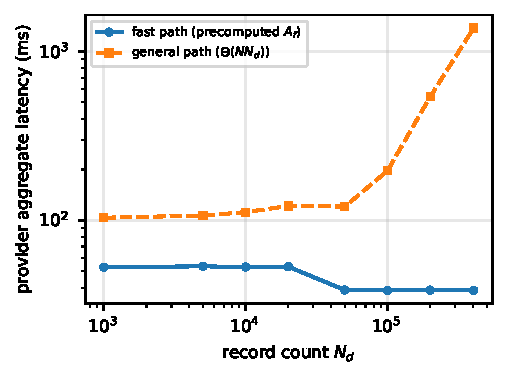
\includegraphics[width=0.72\linewidth]{Figures/telemetry/fig_aggregate_latency.pdf}
\caption{Aggregate latency, fast path against the single-round general path
(C++, two-ciphertext layout). The $x$-axis is $N_d$,
not $|S|$: cost no longer depends on the matched-set size. The fast path is
flat to $\pm0.5\%$ over a $405\times$ range.}
\label{fig:complat}
\end{figure}
\begin{table}[pos=htbp]
\caption{Aggregate latency and storage, fast path against the single-round
general path, $N=11{,}580$, template \textsc{sum}, C++ prototype,
two-ciphertext layout. Medians of $11$ runs (fast) and $3$ (general).}
\label{tab:compute}
\centering
\footnotesize
\setlength{\tabcolsep}{3pt}
\renewcommand{\arraystretch}{1.2}
\begin{tabular*}{\tblwidth}{@{\extracolsep{\fill}}lcccc@{}}
\toprule
$N_d$ & Fast & General & $I'$ / provider & Downlink \\
      & (ms) & (ms)     & (GB)            & (B) \\
\midrule
$10^3$             & $38.8$ & $103.7$   & $0.09$  & $525{,}950$ \\
$5\times10^3$      & $39.0$ & $106.9$   & $0.46$  & $525{,}950$ \\
$10^4$             & $38.8$ & $111.9$   & $0.93$  & $525{,}950$ \\
$2\times10^4$      & $38.8$ & $121.7$   & $1.85$  & $525{,}950$ \\
$5\times10^4$      & $39.1$ & $120.7$   & $4.63$  & $525{,}950$ \\
$10^5$             & $39.2$ & $196.8$   & $9.26$  & $525{,}950$ \\
$2\times10^5$      & $39.1$ & $539.5$   & $18.53$ & $525{,}950$ \\
$4.05\times10^5$   & $38.8$ & $1{,}378.2$ & $37.54$ & $525{,}950$ \\
\bottomrule
\end{tabular*}
\end{table}

\subsection{Comparison against baselines}
Table~\ref{tab:baselines} places the C++ fast path against the baselines on
the primary corpus for a probe tag with the median $|S|=35$. Plaintext scan and
single-server searchable encryption are essentially free and leak everything
or the access pattern and $|S|$; Path ORAM pays per matched record, so its cost
and $373$\,kB downlink scale with $|S|$. The DORY-style search-only baseline
costs $130.4$\,ms, $3.3\times$ the fast path, because it materialises the
selection vector the fast path never touches. The faithful homomorphic
equality scan needs multiplicative depth $17$ at ring dimension $32{,}768$:
$1.86$\,s per batch of $32{,}768$ slots and $24.2$\,s per query, extrapolated,
$617\times$ the fast path. It is the right comparison for ad-hoc predicates on
one server; for registered aggregates the stronger single-server alternative is
baseline~(vi), measured in Section~\ref{sec:packresult}.

\begin{table}[pos=htbp]
\caption{Baselines, same corpus and machine, $N_d=10^5$, probe tag with the
median $|S|=35$. $\dagger$ marks an extrapolated value.}
\label{tab:baselines}
\centering
\footnotesize
\setlength{\tabcolsep}{3pt}
\renewcommand{\arraystretch}{1.2}
\begin{tabular}{@{}lcc>{\raggedright\arraybackslash}p{2.1cm}@{}}
\toprule
System & Server & Downlink & Leakage to the \\
       & (ms)   & (B)      & server(s) \\
\midrule
Plaintext scan        & $<0.001$ & $8$              & everything \\
SSE, 1 server         & $<0.001$ & $560$            & search and access
pattern, $|S|$ \\
Path ORAM             & $0.059^{\dagger}$ & $373{,}248$ & $|S|$, via access
count \\
DORY-style search     & $130.4$  & $800{,}000$      & none; no analytics \\
FHE equality scan     & $24{,}157^{\dagger}$ & n/a & none; 1 server \\
\midrule
\textbf{CR-SHE, fast} & $\mathbf{39.2}$ & $\mathbf{525{,}950}$ &
$\mathrm{class}(q)$ only \\
\bottomrule
\end{tabular}
\end{table}

\subsection{Response packing, and what the trust split buys}
\label{sec:packresult}
Table~\ref{tab:packing} puts the two-ciphertext layout, the packed layout of
Section~\ref{sec:packing}, its compressed form and four-template responses
through the reference implementation at both corpora's tag domains, together
with baseline~(vi), a single server holding the same encrypted columns. All
rows come from one implementation on one machine and one thread, so they
compare with each other and not with the C++ figures. Byte counts are a
property of the parameters and of OpenFHE's serialisation, not of the
machine; the C++ prototype's $262{,}975$\,B per ciphertext against
$263{,}011$\,B here is a serialisation-version difference.

\begin{table}[pos=htbp]
\caption{Fast path per provider: two-ciphertext against packed layouts, and a
single server on the same columns (baseline vi). Reference implementation,
one thread; medians of 21 runs. $k$ is the number of templates answered.}
\label{tab:packing}
\centering
\footnotesize
\setlength{\tabcolsep}{3pt}
\begin{tabular*}{\tblwidth}{@{\extracolsep{\fill}}lccc@{}}
\toprule
Layout & $k$ & Provider (ms) & Downlink (B) \\
\midrule
% --- generated from results/*.json by bench/make_tables.py ---
\multicolumn{4}{@{}l}{\emph{$N=11{,}580$ tags}} \\
Two ct (unpacked) & $1$ & $53.0$ & $526{,}022$ \\
Packed, 1 ct & $1$ & $23.5$ & $263{,}011$ \\
Packed + compressed & $1$ & $27.0$ & $132{,}081$ \\
$4\times$ two ct & $4$ & $194.9$ & $2{,}104{,}088$ \\
Packed, 1 ct & $4$ & $35.4$ & $263{,}011$ \\
Packed + compressed & $4$ & $32.7$ & $132{,}081$ \\
Single server (vi) & $1$ & $42.6$ & $263{,}211$ \\
\midrule
\multicolumn{4}{@{}l}{\emph{$N=35{,}162$ tags}} \\
Two ct (unpacked) & $1$ & $55.8$ & $526{,}022$ \\
Packed, 1 ct & $1$ & $31.4$ & $263{,}011$ \\
Packed + compressed & $1$ & $36.4$ & $132{,}081$ \\
$4\times$ two ct & $4$ & $245.6$ & $2{,}104{,}088$ \\
Packed, 1 ct & $4$ & $74.2$ & $263{,}011$ \\
Packed + compressed & $4$ & $92.3$ & $132{,}081$ \\
Single server (vi) & $1$ & $92.5$ & $263{,}211$ \\
\bottomrule
% ---
\end{tabular*}
\end{table}

\emph{Packing halves the provider's work and the downlink.} One rotate-and-sum
over half-rows replaces two over full rows: a single template falls from
$53.0$ to $23.5$\,ms at $N=11{,}580$ and from $55.8$ to $31.4$\,ms at
$N=35{,}162$, and the response from two ciphertexts to one, $263{,}011$\,B, or
$132{,}081$\,B compressed. Four templates in one compressed response cost
$32.7$\,ms and $132{,}081$\,B at $N=11{,}580$, against $194.9$\,ms and
$2{,}104{,}088$\,B for four two-ciphertext responses ($16\times$ less downlink).
At $N=35{,}162$ they need $35$ chunks instead of $12$, so the cost grows to
$74$--$92$\,ms while the response stays one ciphertext.

\emph{Against a single server, the trust split buys the client side.}
Baseline~(vi) needs no non-collusion assumption. Its server costs $42.6$ and
$92.5$\,ms at the two tag domains, $1.8$ and $2.9$ times one packed CR-SHE
provider ($23.5$ and $31.4$\,ms), because its contraction multiplies ciphertext
by ciphertext; its response is the same one ciphertext. The ratios compare one
provider with one server: two CR-SHE providers together spend $47.0$ and
$62.8$\,ms, so in total server work the trust split costs more than a single
server at the smaller tag domain and saves about a third at the larger. Its query is not (Table~\ref{tab:uplink}):
$789{,}033$ and $2{,}367{,}099$\,B of fresh ciphertexts against a $260$ or
$294$\,B DPF key per provider ($520$ and $588$\,B in total for two),
$3{,}035$ and $8{,}051$ times more uplink per provider, and $14.6$ and
$67.5$\,ms of client encryption against $0.54$ and $0.62$\,ms of key
generation. Query compression by ciphertext expansion \citep{angel2018pir}
would cut that uplink to one ciphertext for more server automorphisms; we did
not implement it.

\begin{table}[pos=htbp]
\caption{Per-query uplink and client cost: CR-SHE's two-party key against the
single server's encrypted query. Reference implementation, one thread.}
\label{tab:uplink}
\centering
\footnotesize
\setlength{\tabcolsep}{3pt}
\begin{tabular*}{\tblwidth}{@{\extracolsep{\fill}}lcccc@{}}
\toprule
 & Key (B) & Enc.\ query (B) & Cts & Encrypt (ms) \\
\midrule
% --- generated from results/*.json by bench/make_tables.py ---
$N=11{,}580$ & $260$ & $789{,}033$ & $3$ & $14.6$ \\
$N=35{,}162$ & $294$ & $2{,}367{,}099$ & $9$ & $67.5$ \\
% ---
\bottomrule
\end{tabular*}
\end{table}

On retrieval a single server must bring every word of the packed
$N\times\lceil N_d/32\rceil$ index into contact with an encrypted one-hot
query, about $\lceil N\lceil N_d/32\rceil/\ell\rceil$ plaintext-ciphertext
products in a direct packed-selection formulation; query compression,
preprocessing or specialised PIR layouts may change that. At the measured
$0.092$\,ms per product this estimate is $81.6$\,ms at
$N_d=2\times10^4$ and $1.65$\,s at $N_d=405{,}184$, against $26.0$\,ms and
$1.10$\,s for CR-SHE's packed retrieval (Table~\ref{tab:packed}); across the
sweep the ratio is $1.5$--$3.1\times$ for that cost model, not against a
measured optimised single-server system, and the two figures come from separate
runs. The separation on every single-keyword path is therefore a small constant
factor in server work, set by a homomorphic slot operation ($11$\,ns here)
against a word operation, plus three orders of magnitude in uplink. That is the
honest case for the non-collusion assumption on these paths: it pays where the
client is thin or the link is metered, which is the IoT setting. On ranges
(Section~\ref{sec:rangeresult}) the gap is wider.

\subsection{The flexible path}
\label{sec:flexresult}
Table~\ref{tab:flex} reports the two rounds of a flexible query at
$N=11{,}580$ in the reference implementation, swept in decreasing $N_d$ to
control for warm-up. Round one, the retrieval, grows linearly with $N_d$ as
its $\Theta(NN_d)$ contraction predicts. Round two costs $20.1$--$35.6$\,ms
with no trend in $N_d$ over this range, because one to five packed products are
dwarfed by the twelve rotations of the row sum, and it returns one
$132{,}081$\,B ciphertext whatever the selection. Its uplink is a $16$\,B seed
to $n-1$ providers and $8N_d$\,B to one. Every flexible query in the reference implementation's tests, including
conjunctions, disjunctions and ad-hoc weights, decrypts to the plaintext ground
truth.

\begin{table}[pos=htbp]
\caption{Flexible path, $N=11{,}580$, $n=2$, reference implementation, one
thread. Round-two uplink is the heavy provider's; the others receive 16\,B.}
\label{tab:flex}
\centering
\footnotesize
\setlength{\tabcolsep}{2pt}
\begin{tabular*}{\tblwidth}{@{\extracolsep{\fill}}lccccc@{}}
\toprule
$N_d$ & Round 1 & Round 2 & Up (B) & Down (B) & $I'$ \\
      & (ms)    & (ms)    &        &          & (GB) \\
\midrule
% --- generated from results/*.json by bench/make_tables.py ---
$1{,}000$ & $41.2$ & $20.1$ & $8{,}000$ & $132{,}081$ & $0.09$ \\
$5{,}000$ & $247.3$ & $35.6$ & $40{,}000$ & $132{,}081$ & $0.46$ \\
$10{,}000$ & $399.4$ & $21.9$ & $80{,}000$ & $132{,}081$ & $0.93$ \\
$20{,}000$ & $758.0$ & $26.4$ & $160{,}000$ & $132{,}081$ & $1.85$ \\
% ---
\bottomrule
\end{tabular*}
\end{table}

\subsection{Packed masked index}
\label{sec:packedresult}
Table~\ref{tab:packed} compares the masked index with one membership bit per
$\mathbb{Z}_p$ word against $32$ bits per word, at the primary corpus's tag
domain $N=11{,}580$, in the reference implementation. Packing divides the index
by exactly $32$ and makes retrieval $19$ to $27$ times faster at
$N_d=10^4$ and $2\times10^4$, where both layouts fit in this machine's memory.
At the full $405{,}184$ records the packed index is $1.17$\,GB, against
$37.5$\,GB unpacked (computed), and a retrieval takes $1.10$\,s and returns
$101{,}296$\,B per provider. Every retrieval returned exactly the posting list.

\begin{table}[pos=htbp]
\caption{Masked index, unpacked against $32$ bits per word, $N=11{,}580$.
Reference implementation, one thread; retrieval per provider.}
\label{tab:packed}
\centering
\footnotesize
\begin{tabular*}{\tblwidth}{@{\extracolsep{\fill}}llccc@{}}
\toprule
$N_d$ & Layout & Index (GB) & Retrieval (ms) & Downlink (B) \\
\midrule
\inputtbl tables/packed.tex 
\bottomrule
\end{tabular*}
\end{table}

\subsection{Multi-cloud deployment}
\label{sec:wanresult}
With $n\in\{2,3,4\}$ separate provider processes and a client over TCP on one
host (Table~\ref{tab:wan}), provider compute is flat in $n$, at $34.82$,
$34.85$ and $35.48$\,ms, so the client waits on the slowest provider, not on
their sum. End-to-end latency rises from $44.1$ to $52.5$\,ms, all of it
transport of the $n$ responses; the client's combine, verify and decrypt cost
$1.37$--$1.63$\,ms. The transport covers loopback only: wide-area latency,
bandwidth variation, stragglers and recovery were not measured, so no fixed
cross-region increment can be inferred from these figures.

\begin{table}[pos=htbp]
\caption{Single-host deployment over loopback, medians of 100 queries.
Transport excludes wide-area latency.}
\label{tab:wan}
\centering
\footnotesize
\setlength{\tabcolsep}{3pt}
\renewcommand{\arraystretch}{1.2}
\begin{tabular*}{\tblwidth}{@{\extracolsep{\fill}}lcccc@{}}
\toprule
$n$ & End-to-end & Provider & Transport & Client \\
    & (ms)       & (ms)     & (ms)      & (ms) \\
\midrule
$2$ & $44.12$ & $34.82$ & $8.30$  & $1.37$ \\
$3$ & $45.40$ & $34.85$ & $9.09$  & $1.52$ \\
$4$ & $52.53$ & $35.48$ & $15.48$ & $1.63$ \\
\bottomrule
\end{tabular*}
\end{table}

\subsection{Communication}
\label{sec:commresult}
At $N=11{,}580$ the two-party construction sends a $266$\,B key to each
provider, $532$\,B of uplink in total. The non-succinct $n$-party
instantiation used for $n>2$ sends $32$\,B to each of $n-1$ providers and
$92{,}656$\,B to one, so total uplink is $92{,}688$\,B at $n=2$,
$92{,}720$\,B at $n=3$ and $92{,}752$\,B at $n=4$. Tolerating more collusion
is therefore nearly free in this instantiation, but moving beyond two
providers at all costs a factor of $174$ in uplink over the succinct two-party
tree. A succinct
$(n{-}1)$-private instantiation would reduce the heavy key from $O(N\log p)$
to $O(2^{n/2}\sqrt{N}\lambda)$.


Downlink is $525{,}950$\,B per provider for an aggregate in the two-ciphertext
layout and $132{,}081$\,B packed and compressed, for up to four templates in
our configuration, and a fixed $\lceil N_d/32\rceil$ words for a retrieval,
which is $25{,}000$\,B at $N_d=10^5$ packed ($800{,}000$\,B unpacked), none
depending on $|S|$. A range query and a flexible round each return one
$132{,}081$\,B ciphertext.

\subsection{Leakage evaluation}
\label{sec:leakeval}
We mount a frequency and volume leakage-abuse attack in the style of
\citet{islam2012access} and \citet{cash2015leakage} against our own index,
twice: once against an unmasked replicated index, whose rows expose their
Hamming weight and hence every posting-list length, and once against the
masked index of Section~\ref{sec:mask}, whose row statistics we compute with
the real PRF over all $11{,}580\times405{,}184$ entries. The adversary's
auxiliary knowledge is the tag-frequency distribution of a similar deployment,
modelled by binomially thinning the true posting lengths to a sampled fraction
of the records, so the attack is not handed the answer.

Aggregated over the whole tag universe (Fig.~\ref{fig:leakage}) the unmasked
index yields $4.27\%$ re-identification under perfect auxiliary knowledge,
against $0.0086\%$ for random guessing, a $500\times$ lift but low in absolute
terms. That aggregate is misleading, and Table~\ref{tab:leakage} shows why:
$11{,}523$ of the $11{,}580$ tags are one-minute time buckets of near-identical
length, which volume leakage genuinely cannot separate. Every other tag class,
meaning the device identifiers, the light and motion flags and all five
sensor-band families, is re-identified \emph{completely}, at $100\%$. These
are precisely the tags that carry semantic meaning: which device, which sensor
condition.

\begin{figure}[pos=htbp]
\centering
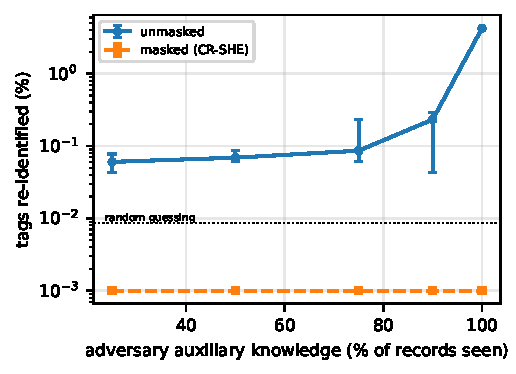
\includegraphics[width=0.72\linewidth]{Figures/telemetry/fig_leakage_attack.pdf}
\caption{Tag re-identification against the unmasked and masked index, against
the adversary's auxiliary knowledge. Table~\ref{tab:leakage} breaks it down by
class.}
\label{fig:leakage}
\end{figure}

Against the masked index the same attack recovers $0.00\%$ in every class and
at every level of auxiliary knowledge. A more demanding comparison is with
the standard padding defences rather than with no defence: padding each
posting list to the next power of two, and volume-hiding padding of every row
to the longest, which on these corpora would inflate posting storage by
$1{,}285\times$ and $778\times$ (computed from the corpus statistics). The
reference implementation provides the same attack against both
(\texttt{bench/bench\_leakage.py}); we have not yet run it on the corpora
(Section~\ref{sec:limits}).\authorcheck{Run bench/bench\_leakage.py on both
corpora and add the padded and volume-hiding columns to
Table~\ref{tab:leakage}; the raw files could not be fetched where the reference
results were produced.}
The masked row statistics are not
distinguishable from uniform over $\mathbb{Z}_p$ by a $64$-bin chi-square test
($\chi^2=72.27$ on $63$ degrees of freedom, $p_{\chi^2}=0.198$). This is the
empirical counterpart of Theorem~\ref{thm:mask}, evidence for it rather than a
proof of it. We note that this experiment is deterministic given the corpus
and the key seed, and reproduced to the digit on two different machines and
microarchitectures. Section~\ref{sec:secondcorpus} repeats the attack on a
twelve-site corpus with three times the tag domain and obtains the same
per-class picture, so neither the $100\%$
unmasked recovery nor the $0\%$ masked recovery is an artefact of this
corpus's three devices.

\begin{table}[pos=htbp]
\caption{Tag re-identification by metadata class, primary corpus, under
perfect auxiliary knowledge.}
\label{tab:leakage}
\centering
\footnotesize
\setlength{\tabcolsep}{3pt}
\renewcommand{\arraystretch}{1.15}
\begin{tabular*}{\tblwidth}{@{\extracolsep{\fill}}lccc@{}}
\toprule
Tag class & Tags & Unmasked & Masked \\
\midrule
Device identifier      & $3$      & $100\%$ & $0\%$ \\
Light flag             & $2$      & $100\%$ & $0\%$ \\
Motion flag            & $2$      & $100\%$ & $0\%$ \\
CO band                & $10$     & $100\%$ & $0\%$ \\
Humidity band          & $10$     & $100\%$ & $0\%$ \\
LPG band               & $10$     & $100\%$ & $0\%$ \\
Smoke band             & $10$     & $100\%$ & $0\%$ \\
Temperature band       & $10$     & $100\%$ & $0\%$ \\
One-minute window      & $11{,}523$ & $3.80\%$ & $0\%$ \\
\midrule
Random guessing        & n/a      & \multicolumn{2}{c}{$0.0086\%$} \\
\bottomrule
\end{tabular*}
\end{table}

\subsection{Setup, masking and ingest costs}
\label{sec:setupresult}
Unpacked, the mask costs a factor of $64$ in index storage over a plaintext
bitmap; packed, a factor of $2$. In the C++ prototype the unpacked masked index
at $N_d=10^5$ took $5.6$\,s to build, the fast-path column $A_f$ $1.2$--$12$\,ms
per template, occupying $2$ ciphertexts ($0.53$\,MB) whatever $N_d$, and a
complete provider bundle for the full corpus (context, evaluation keys, $pk$
and eight columns) was $12$\,MB and took $0.8$\,s to produce. Insertion into the hot
buffer ran at $4.5$--$14.1$ million records per second; a fast-path static-tier
rebuild cost $14.7$--$14.9$\,ms per template, $58.0\,\mu$s per insertion at
$B=256$ and $0.91\,\mu$s at $B=16{,}384$, while the buffer scan added
$98.8$--$100.0\%$ to a query. The range cube registered in
Section~\ref{sec:rangeresult} took $1.3$\,s (combined) and $9.8$\,s
(per-corner) to build and encrypt in the reference implementation.
\authorcheck{Re-measure the masked-index build with rejection sampling and
packing in C++.}


\subsection{Core scaling and throughput}
\label{sec:scaling}
In the C++ prototype a single fast-path query does not speed up with cores
($34.3$, $34.4$ and $38.4$\,ms at $1$, $8$ and $64$ threads), because the
homomorphic contraction dominates, but throughput does: $29.1$ queries/s with
one client, $56.9$ with two, $110.2$ with four, and a plateau of
$121.6$--$127.7$ from sixteen to sixty-four clients, with median latency rising
from $34.4$ to $516$\,ms; between four and sixteen clients throughput is within
$15\%$ of its maximum and median latency stays under $135$\,ms.

\subsection{Tamper evidence}
\label{sec:verifyresult}
Table~\ref{tab:verify} injects five provider deviations, $200$ trials each, into
every path and every verification mode of the reference implementation; one
provider deviates and the other is honest. The last deviation is the strongest
we can stage: the provider perturbs exactly the point the query reads, as if it
knew the query. The fast path uses $N=11{,}580$ tags, the range path a
$3\times200\times10$ cube, the flexible round $4{,}096$ records and retrieval a
$512$-tag index.

\begin{table}[pos=htbp]
\caption{Detected / undetected-and-wrong over $200$ trials per cell, by path
and verification mode. Columns: a constant added to the value slot; the share
plus a uniform vector; the share scaled by $k$; the share plus $c\,u_x$ at a
random point; the same at the point the query reads. Trials not counted were
undetected and left the answer unchanged (the perturbed row was empty).
Reference implementation.}
\label{tab:verify}
\centering
\footnotesize
\setlength{\tabcolsep}{3pt}
\begin{tabular*}{\tblwidth}{@{\extracolsep{\fill}}llccccc@{}}
\toprule
Path & Check & Constant & Uniform & Scale & Random pt & Queried pt \\
\midrule
\inputtbl tables/verify.tex 
\bottomrule
\end{tabular*}
\end{table}

\emph{One stored key} catches only the inconsistent constant: every consistent
substitution, on every path, was accepted with a wrong answer, $0/200$ detected
in each cell. The C++ prototype gave the same $200/200$ and $0/200$ on the fast
path. \emph{Per-position keys} catch every deviation except the one aimed at
the queried point, which passed $200$ times out of $200$ on the fast path and
on the range path alike; they exist on neither the flexible path nor
retrieval. \emph{The session check} detected every deviation that changed the
answer: across the $4{,}000$ session trials on the four paths no wrong answer
was accepted, and the $32$ undetected fast-path trials perturbed an empty row,
so their answers were correct. Retrieval without it relies on the four spare
bits of each packed word, which catch any deviation that scrambles words but
missed a single flipped membership bit in all $200$ trials; the session check
caught all of them.

\subsection{Role-scoped access}
\label{sec:authresult}
Table~\ref{tab:roles} repeats the extraction attack of our earlier
measurement, in which a client sending raw additive shares of basis vectors
read every row of the masked index undetected (the C++ prototype recovered
$512$ of $512$ rows). The reference deployment has $512$ tags over three roles
of $4{,}096$ records each; the attacker holds role~$0$ and sends a raw share
vector for every row. With one mask key it recovers every row exactly, including
all $365{,}227$ membership bits that belong to the other two roles. With
role-scoped keys it recovers none of those bits and no row exactly; when it
applies its own key to the other roles' words, $6.06\%$ of them pass the width
check, against the $6.25\%$ expected of uniform words. Through the fast path the
same user obtained, for all $512$ tags, exactly the role-$0$ aggregate and in no
case the all-role one, and a flexible round asking for every record returned
the role-$0$ total. The price is storage: the aggregate columns, cube tables and
record column are held once per role, while the masked index, the largest
structure, is shared.

\begin{table}[pos=htbp]
\caption{Index extraction by a role-$0$ user sending raw shares for all
$512$ rows; three roles of $4{,}096$ records. Reference implementation.}
\label{tab:roles}
\centering
\footnotesize
\begin{tabular*}{\tblwidth}{@{\extracolsep{\fill}}lccc@{}}
\toprule
Index & Rows exact & Other roles' bits & Other words \\
 & & recovered & pass width check \\
\midrule
\inputtbl tables/roles.tex 
\bottomrule
\end{tabular*}
\end{table}

\subsection{Second corpus: twelve sites and a larger tag domain}
\label{sec:secondcorpus}
The primary corpus has three devices, so its tag universe is dominated by time
buckets. The C++ prototype therefore repeated every experiment above on the
Beijing corpus, whose twelve sites give three times the tag domain
($N=35{,}162$, posting lengths median $12$, mean $131.5$, maximum $102{,}344$).
Missing readings get their own \texttt{:na} tag rather than falling into the
lowest band, since CO is missing in $4.92\%$ of records, and temperature is
shifted by $+50\,^\circ$C so that it stays non-negative. Every correctness
check passed unchanged, including a byte-identical $525{,}950$\,B downlink for
$|S|=0$ and $|S|=5{,}000$.

\emph{The fast path is unaffected by the larger tag domain.} It cost
$40.2$--$41.2$\,ms from $N_d=5\times10^3$ to $4.05\times10^5$
(Table~\ref{tab:beijing}), $5\%$ more than on the primary corpus for
$3.04\times$ the tags: the packed products grow from $2$ ciphertexts to $5$,
but the fixed rotate-and-sum, encryption and serialisation dominate. The first
point, $54.6$\,ms at $N_d=10^3$, carries the warm-up artefact of
Section~\ref{sec:aggresult}, since this sweep ran in increasing $N_d$.
\emph{The unpacked masked index is storage-bound.} The general path cost
$382.0$\,ms at $N_d=10^5$ against $196.8$\,ms on the primary corpus, and its
unpacked index grew to $28.13$\,GB; the harness refused the last two points,
which needed $56.26$ and $113.98$\,GB, against a $47.5$\,GB budget. Packing
(Section~\ref{sec:mask}) divides all of these by $32$, to $3.6$\,GB at
$N_d=4.05\times10^5$ (computed).

\begin{table}[pos=htbp]
\caption{Second corpus ($N=35{,}162$, $N_d$ up to $420{,}370$): aggregate
latency and unpacked index size, template \textsc{sum}, C++ prototype,
two-ciphertext layout. Sweep in increasing $N_d$; ``n/a'' marks a point the
harness refused on its memory budget.}
\label{tab:beijing}
\centering
\footnotesize
\setlength{\tabcolsep}{3pt}
\begin{tabular*}{\tblwidth}{@{\extracolsep{\fill}}lcccc@{}}
\toprule
$N_d$ & Fast (ms) & General (ms) & $I'$ (GB) & Downlink (B) \\
\midrule
$10^3$             & $54.6$ & $106.3$ & $0.28$   & $525{,}950$ \\
$5\times10^3$      & $40.4$ & $86.9$  & $1.41$   & $525{,}950$ \\
$10^4$             & $40.2$ & $99.7$  & $2.81$   & $525{,}950$ \\
$2\times10^4$      & $40.5$ & $145.5$ & $5.63$   & $525{,}950$ \\
$5\times10^4$      & $40.7$ & $220.8$ & $14.06$  & $525{,}950$ \\
$10^5$             & $41.2$ & $382.0$ & $28.13$  & $525{,}950$ \\
$2\times10^5$      & $40.9$ & n/a     & $56.26$  & $525{,}950$ \\
$4.05\times10^5$   & $40.9$ & n/a     & $113.98$ & $525{,}950$ \\
\bottomrule
\end{tabular*}
\end{table}

\emph{The leakage conclusion is not an artefact of three devices.} The
unmasked index again gave up every one of the ten non-temporal tag classes at
$100\%$, including the twelve sites and seventeen wind directions, and the
hour buckets at $0.31\%$; the masked index gave up $0.00\%$ in every class,
its row sums indistinguishable from uniform ($\chi^2=62.38$ on $63$ degrees of
freedom, $p_{\chi^2}=0.4986$; Table~\ref{tab:leakagebeijing}).

\begin{table}[pos=htbp]
\caption{Tag re-identification by class, second corpus, perfect auxiliary
knowledge.}
\label{tab:leakagebeijing}
\centering
\footnotesize
\setlength{\tabcolsep}{3pt}
\begin{tabular*}{\tblwidth}{@{\extracolsep{\fill}}lccc@{}}
\toprule
Tag class & Tags & Unmasked & Masked \\
\midrule
Monitoring site        & $12$       & $100\%$   & $0\%$ \\
Wind direction         & $17$       & $100\%$   & $0\%$ \\
CO, NO$_2$, O$_3$ bands & $33$      & $100\%$   & $0\%$ \\
PM$_{2.5}$, PM$_{10}$ bands & $22$  & $100\%$   & $0\%$ \\
SO$_2$ band            & $10$       & $100\%$   & $0\%$ \\
Pressure, dew-point bands & $22$    & $100\%$   & $0\%$ \\
One-hour window        & $35{,}046$ & $0.31\%$  & $0\%$ \\
\midrule
Random guessing        & n/a        & \multicolumn{2}{c}{$0.0028\%$} \\
\bottomrule
\end{tabular*}
\end{table}

\emph{The remaining measurements track the primary corpus.} Provider compute
in the single-host deployment was flat in $n$ ($38.67$, $37.65$ and
$38.47$\,ms for $n=2,3,4$), with end-to-end latency rising from $48.17$ to
$56.04$\,ms in transport alone. The DORY-style search-only baseline cost
$305.6$\,ms against $41.2$\,ms for the complete fast path, so the gap widens to
$7.4\times$ as $N$ grows; the homomorphic equality scan, $24.4$\,s, is
essentially unchanged, $592\times$ the fast path. Throughput plateaued at
$117$--$124$ queries/s; insertion into the hot buffer ran at $4.5$--$11.1$
million records per second; a fast-path static-tier rebuild cost
$28.7$--$29.1$\,ms, twice the primary corpus and linear in $N$; and building
the unpacked masked index at $N_d=10^5$ took $16.6$\,s against $5.6$\,s, while
$A_f$ stays $5$ ciphertexts ($1.3$\,MB). Selection latency and keys depend on
$N$ alone and were not re-measured: the two-party key is $300$\,B and the
$n$-party heavy key $8N+16=281{,}312$\,B, both computed.

\subsection{Discussion}
\emph{Ranges are where the design pays.} A registered range aggregate costs the
same for a one-minute window as for the whole timeline and returns one
ciphertext; the single-tag path would need one query per cell, the flexible
path one retrieval per tag, and a single server an encrypted query as long as
the cube. On single-keyword aggregates one CR-SHE provider is $1.8$--$2.9$
times faster than a single server holding the same columns, but two providers
together are not, so the trust split's case rests on the client side: on
ranges the uplink gap reaches four orders of magnitude, $5.5$\,kB verified
against a computed $44$\,MB, which is the regime a thin IoT client is in.

\emph{Verification no longer costs a layout.} With stored keys the choice was
between the combined layout, cheap and unverifiable against consistent
substitution, and the per-corner layout, eight times the storage and still
blind to the queried corner. The per-query secret removes the trade: the
verified layout keeps the combined layout's storage and homomorphic work,
catches every deviation we injected that changed an answer, and costs one more
full-domain evaluation per key.

\emph{Cube size is the provisioning knob.} Range cost grows linearly in the
number of cells, $1.36$\,s per provider at $10^6$ cells in the combined layout
of our unoptimised implementation. A deployment registers the cubes its
analysts need, as it registers templates and roles, and the cell count, not the
record count, bounds the per-query cost.

\emph{Retrieval is bounded by time, not storage.} Packing brings the masked
index from $37.5$ to $1.17$\,GB per provider at the full primary corpus, so the
flexible path, which serves arbitrary selections in two rounds, fits on
commodity hosts.

\subsection{Limitations}
\label{sec:limits}
\emph{Evaluation.} Range aggregation, session verification, role-scoped access
and the packed index were measured in a single-threaded reference
implementation on synthetic data with the primary corpus's dimensions, not in
the C++ prototype on the real corpora; absolute latencies are those of an
unoptimised driver, and figures are per provider. The C++ deployment ran over
loopback on one host, so wide-area latency, bandwidth variation and stragglers
were not measured, and the padded leakage baselines have not been run.
\authorcheck{Port range aggregation and the session check to the C++ build,
measure them on both real corpora, run the padded leakage baselines, and deploy
providers in at least two cloud regions.}

\emph{Expressiveness and updates.} One-round range queries apply to registered
data cubes and templates whose cumulative corpus total stays below $p$ (a
corpus-wide sum of squares requires a larger plaintext modulus $p$), while
non-rectangular predicates and cross-cube conjunctions use the two-round
flexible path.

\emph{Adversary.} Privacy is proved for semi-honest providers and a trusted
owner. Tamper evidence holds against arbitrary provider deviation but gives no
output delivery, and a DU that reveals its aborts can leak up to one bit about
the data per query. Role confinement assumes providers apply the policy and do
not collude with users; it covers record partitions, not per-tag rights within
a role.

\emph{Collusion beyond two providers.} For $n>2$ the prototype uses a
non-succinct sharing whose heavy key is $8N+16$ bytes; a range query needs
$2^d$ such keys over the cube's $M$ cells, twice that verified. Our key-size
claims are for $n=2$.

\emph{Prior art.} Private aggregation, prefix-sum cubes and encrypted range
aggregates are established topics, and Obscure is close on oblivious,
verifiable, non-interactive aggregation. The $2^d$ box decomposition, the
one-time-padded index and the client-chosen one-time MAC key each have a
direct precursor \citep{boyle2016function,dory,li2026silent}; what we offer is
their combination in this setting. Our statements about Obscure, Hafiz et al.\
and HADES rest on abstracts and search summaries, and a like-for-like
comparison with them remains to be done.

\emph{Multi-owner extensions.} The construction assumes a single data owner
and full delegation of decryption within each role; extending ingestion to
multiple independent data owners via multi-key or threshold homomorphic
encryption is a natural next step.

\section{Conclusion}
\label{sec:conclusion}

IoT analytics are range aggregates over time, place and value, and the data
behind them increasingly sit encrypted across several clouds. CR-SHE answers
such aggregates in one round, over data encrypted under one owner's key,
hiding the range, the matched records, their number and the result from any
coalition of up to $n-1$ providers that never talk to one another. Encrypted
summed-area tables turn any box of a registered cube into $2^d$ point
selections whose signs and dummy padding hide the box; oblivious homomorphic
aggregation contracts each provider's share against encrypted columns so that
the matched set is never assembled; a secret scalar drawn afresh for each query
and carried in the keys makes any answer-changing deviation evident to the
client at no extra homomorphic cost; and role-scoped columns and mask keys
confine each user to its own records without interaction. At $t=n-1$ a
homomorphic layer is our route to this, since a local additive-sharing
alternative with data-independent queries would need single-server private
retrieval. On two real IoT corpora a C++ prototype answers single-keyword
aggregates in $39$\,ms per provider; on a synthetic cube with the primary
corpus's dimensions a reference implementation returns fixed-size
$132$\,kB responses at flat cost across box lengths, accepted no wrong answer
in $4{,}000$ tampered session queries, and leaked no other role's records under
an index-extraction attack. Range results on the real corpora, a native port,
cross-region latency and an outside review of the proofs come next.
Future work will pursue sublinear preprocessing for dynamic streams,
succinct multi-party DPF instantiations for $n>2$, wide-area multi-region and
edge-gateway evaluations, and multi-owner key management.

% ===========================================================================
% \printcredits emits its own "CRediT authorship contribution statement"
% heading from the \credit declarations in the front matter.
\ifanonymous\else\printcredits\fi

\section*{Declaration of competing interest}
The authors declare that they have no known competing financial interests or
personal relationships that could have appeared to influence the work reported
in this paper.

\section*{Acknowledgements}
This research did not receive any specific grant from funding agencies in the
public, commercial, or not-for-profit sectors.

\section*{Data availability}
Data will be made available on request.

\section*{Declaration of generative AI and AI-assisted technologies in the
manuscript preparation process}
During the preparation of this work the authors used three AI assistants.
Claude (Anthropic) was used to convert the manuscript between journal
templates, edit and restructure the text, write the plotting script that draws
Fig.~\ref{fig:arch}, develop the reference implementation with its tests and
benchmark scripts, search the literature for prior work and compare the
manuscript with papers the authors supplied, and draft parts of
the text and analysis, including the range construction, the tamper-evidence
mechanism with Theorem~\ref{thm:tamper}, role-scoped access with
Proposition~\ref{prop:role}, and Sections~\ref{sec:whyrep}, \ref{sec:flex},
\ref{sec:packing}, \ref{sec:resultsdisc} and~\ref{sec:conclusion}. ChatGPT
(OpenAI) and Gemini (Google) were used to edit and review intermediate drafts;
the framing, corrections, algorithm and proof refinements adopted from them
were checked against the implementation and the measured results, and the
per-record coupled MAC and role-blinded columns they proposed were
reimplemented and measured before inclusion. No image was generated or altered
by a generative AI tool. After using these tools, the authors reviewed and
edited the content as needed and take full responsibility for the content of
the publication.

% ===========================================================================
\bibliographystyle{model1-num-names}
\bibliography{references}

\end{document}
